\documentclass[a4paper, 12pt, openright, oneside, final]{book}%{scrbook}
\usepackage{eso-pic}
\usepackage{float}
\usepackage{graphicx}
\usepackage{setspace}
\usepackage[english]{babel}
\usepackage{listings}
\usepackage{varioref}
\usepackage{subfigure}
\usepackage{verbatim}
\usepackage{amsmath}
\usepackage[pdftex,bookmarks=true,hypertexnames=true]{hyperref}
\usepackage{fancyhdr}
\newcommand{\fncyblank}{\fancyhf{}}
\newcommand{\HRule}{\rule{\linewidth}{0.5mm}}
\newenvironment{abstract}%
{\cleardoublepage\fncyblank\null\vfill\begin{center}%
\bfseries\abstractname\end{center}}%
{\vfill\null}

%\lstset{%
%  basicstyle=\small,
%  frame=tb,
%  captionpos=b,
%  stringstyle=\ttfamily,
%  showstringspaces=false,
%  numbers=left,
%  numberstyle=\tiny,
%  framextopmargin=2pt,
%  framexbottommargin=2pt,
%  stepnumber=1,
%  numbersep=5pt}

\usepackage{courier}
\usepackage{color}
\usepackage{xcolor}
\lstset{
         basicstyle=\footnotesize\ttfamily, % Standardschrift
         %numbers=left,               % Ort der Zeilennummern
         numberstyle=\tiny,          % Stil der Zeilennummern
         %stepnumber=2,               % Abstand zwischen den Zeilennummern
         numbersep=5pt,              % Abstand der Nummern zum Text
         tabsize=2,                  % Groesse von Tabs
         extendedchars=true,         %
         breaklines=true,            % Zeilen werden Umgebrochen
         keywordstyle=\color{red},
 %        frame=b,         
 %        keywordstyle=[1]\textbf,    % Stil der Keywords
 %        keywordstyle=[2]\textbf,    %
 %        keywordstyle=[3]\textbf,    %
 %        keywordstyle=[4]\textbf,   \sqrt{\sqrt{}} %
         stringstyle=\color{black}\ttfamily, % Farbe der String
         showspaces=false,           % Leerzeichen anzeigen ?
         showtabs=false,             % Tabs anzeigen ?
         xleftmargin=5pt,
         framexleftmargin=5pt,
         framexrightmargin=5pt,
         framexbottommargin=4pt,
         %backgroundcolor=\color{lightgray},
         showstringspaces=false      % Leerzeichen in Strings anzeigen ?        
}
\lstloadlanguages{% Check Dokumentation for further languages ...
         %[Visual]Basic
         %Pascal
         C
         %C++
         %XML
         %HTML
         %Java
}
%\DeclareCaptionFont{blue}{\color{blue}} 

\usepackage{caption} \DeclareCaptionFont{white}{\color{white}}
\DeclareCaptionFormat{listing}{\colorbox[cmyk]{0.43, 0.35,
0.35,0.01}{\parbox{\textwidth}{\hspace{15pt}#1#2#3}}}
\captionsetup[lstlisting]{format=listing,labelfont=white,textfont=white,
singlelinecheck=false, margin=0pt, font={bf,footnotesize}}

\hypersetup{
pdfauthor= {Sun Youcheng},
pdftitle= {Design and Development of Real-Time Multi-Processor Bandwidth
Control Mechanisms in General Purpose Operating Systems},
pdfsubject= {Design and Development of Real-Time Multi-Processor Bandwidth
Control Mechanisms in General Purpose Operating Systems},
pdfkeywords = {realtime, scheduling, linux, multiprocessor, hierarchy},
pdfborder = { 0 0 0 0 }
}

%
% TODO: it is better to use title and author keywords here
%
\title{Design and Development of Real-Time Multi-Processor Bandwidth
  Control Mechanisms in General Purpose Operating Systems}

\author{Youcheng Sun}

\onehalfspacing

\begin{document}

\frontmatter

%\maketitle

%\thispagestyle{empty}
\begin{center}
\begin{figure}[htbp]
        \centering
        
\includegraphics[width=\textwidth]{images/logo}
\end{figure}
%\vspace*{0.5in}
\vskip5mm
\textsc{{\bf\large G}RADUATE {\bf\large P}ROGRAM IN {\bf\large C}OMPUTER 
	{\bf\large S}CIENCE AND {\bf\large E}INGINEERING} \\
\hrulefill \\%[0.2cm] 
\text{Master Thesis}%\\[0.8in]
%\vskip12mm
\vfill
% Title
\textsc{ %\large \bfseries 
\textbf{\huge Design and Development of Real-Time Multi-Processor Bandwidth
	Control Mechanisms in General Purpose Operating Systems\\}
}
\vfill
\vskip20mm

\begin{tabular*}{\textwidth}{@{\extracolsep{\fill}}lcr}
Supervisors:                        & \hfill & Candidate: \\
& & \\
Prof. Giuseppe Lipari                & \hfill & Sun Youcheng\\
\emph{\scriptsize Scuola Superiore Sant'Anna } & \hfill & \\
& & \\
%& & \\
Prof. Luca Abeni   & \hfill & \\
\emph{\scriptsize University of Trento }        & \hfill & \\
& & \\
& & \\
\end{tabular*}


\par
Academic year 2011/2012
%\today
\end{center}
%\end{titlepage}

\begin{titlepage}
%\begin{tabular}{c p{3cm} c}
%     \includegraphics[width=114pt]{figures/rwth}
%        & &
%     \includegraphics[width=60pt]{figures/unitn} \\
%     \small \textsc{RWTH Aachen University} & &  \small \textsc{University of Trento}\\
%     \small \textsc{Germany} & & \small \textsc{Italy}
%\end{tabular}

\begin{center}
\vspace*{1in}
\textsc{Master Thesis}\\[0.5cm]

% Title
\HRule \\[0.4cm] 
{ \large \bfseries Design and Development of Real-Time Multi-Processor Bandwidth
	Control Mechanisms in General Purpose Operating Systems
}

%{ \huge \bfseries A Simulation Framework for}\\[0.4cm]
%{ \huge \bfseries Self-Reconfigurable Socio-Technical Systems}\\[0.4cm]
\HRule \\[1.5cm]

%\textbf{Sun Youcheng} \\ [1cm]
%\textit{Supervisors} \\ [1cm]
 \begin{tabular*}{\textwidth}{@{\extracolsep{\fill}}lcr}
    Supervisors:                        & \hfill & Candidate: \\
    & & \\
    Prof. Giuseppe Lipari                & \hfill & Sun Youcheng\\
    \emph{\scriptsize Scuola Superiore Sant'Anna } & \hfill & \\
    & & \\
    %& & \\
    Prof. Luca Abeni   & \hfill & \\
    \emph{\scriptsize University of Trento }        & \hfill & \\
	& & \\
	& & \\
  \end{tabular*}

\begin{figure}[htbp]
        \centering
        
\includegraphics[width=\textwidth]{images/logo}
\end{figure}

%\begin{minipage}{0.45\textwidth}
%\begin{center} \small
%
\includegraphics[width=60pt]{images/logo_trento} \\ %[0.58cm]
%%Prof. Gerhard \textsc{Lakemeyer} \\  
%University of Trento
%%Germany
%\end{center}
%\end{minipage}
%\begin{minipage}{0.45\textwidth}
%\begin{center} \small
%
\includegraphics[width=60pt]{images/logo_sssup} \\
%Scuola Superiore Sant'Anna
%%Prof. Paolo \textsc{Giorgini} \\ 
%%University of Trento \\
%%Italy
%\end{center}
%\end{minipage}



\vfill
Graduate Program in Computer Science and Engineering
\par
\today
\end{center}
\end{titlepage}


\begin{abstract}
  % TODO: the abstract should be a short summary of the contents of
  % the thesis. Very short motivation (the problem to be solved), and
  % what has been done in the thesis.
  % DONE

  %Attentions have been being paid to extend general purpose operating
  %systems with real time functionalities. In this thesis, a scheduling
  %framework, which can control Central Processing Unit (CPU) bandwidth
  %distribution on multi-processor platforms in a real-time way, is
  %proposed in Linux.  Under the framework, cpu bandwidths from
  %different processors are reserved according to Constant Bandwidth
  %Server (CBS) rules.  Yet as for how to utilize the reserved
  %bandwidths to schedule tasks in Linux, this is not the interest of
  %the framework. They can be scheduled by policies used in the Linux
  %system or scheduling algorithms that are implemented for a specific
  %purpose. A subset of these tasks can get a portion of the
  %reservation using the same rule.  Furthermore, under the framework,
  %scheduling policies can be applied in a controlled scale instead of
  %the whole system.

  %In current implementation, both normal tasks and real-time tasks in
  %Linux can work under the framework. Experimental results are not
  %available now ...
  Attentions have been being paid to extend general purpose operating
  systems (GPOS) with real time functionalities. In this thesis, the
  Open-Extension Container(OXC) scheduling framework, which can control 
  Central Processing Unit (CPU) bandwidth distribution on multi-processor 
  platforms in a real-time way, is proposed in Linux. The ox container 
  is a new data structure defined in our work. It has a good feature 
  that from a Linux scheduler's aspect, it behaves as a virtual CPU.  
  Under the framework, cpu bandwidths from different processors are 
  reserved according to Constant Bandwidth Server (CBS) rules.  Yet 
  as for how to utilize the reserved bandwidths to schedule tasks, 
  this is not the interest of the framework. They can be scheduled by 
  policies used in the Linux system or scheduling algorithms that are 
  implemented for a specific purpose. A subset of these tasks can get 
  a portion of the reservation using the same rule.  Furthermore, under 
  the framework, scheduling policies can be applied in a controlled scale 
  instead of the whole system.

  In current implementation, both normal tasks and real-time tasks in
  Linux can work under the framework. Experiments show that our 
  hierarchical CPU bandwidth control is feasible in Linux.
\end{abstract}

\tableofcontents
\listoffigures
\chapter{Introduction\label{chap:introduction}}

Linux is the most widely deployed open source general purpose
operating system. Traditionally, the aim of Linux scheduling is to
distribute cpu cycles fairly among tasks and task groups according to
their relative importance. Because of their popularity and high-level
of compatibility, Linux based systems are used to serve various kinds
of purposes. In some cases, fairness is not enough or necessary.

One important class of applications consists of hard real-time or soft
real-time systems. In order to work well, these applications have
requirements in terms of the CPU cycles they receive, or on the time
they need to react to external events. Such timing guarantee (or
\emph{real-time guarantee}) cannot be provided just by fairness.
Examples of soft real-time applications are multi-media applications.

%%
%% TODO: I do not understand the following sentence 
%%
Indeed, simply from CPU bandwidth management's point of view, a
real-time guarantee is also useful. 
%
In many situations, people prefer to distributing cpu power in a
privileged and predictable way. For instance, to give 10\% of the
total CPU cycles to a set of tasks; furthermore, take half of this
10\% and assign it to a subset of the tasks.

Nowadays, multi-core architectures are successfully used to boost
computing capability for computing devices. Common computing systems
with multiple processors are becoming mainstream: it is no surprise to
see an embedded device with more than one CPU inside.  Yet high speed
processors and more cores rather than solving the CPU timing guarantee
problem do bring more challenges. Also, no matter how powerful the
platform is, there is always time when people need more. So, to fully
utilize multi-core platform is also a good reason to manage computing
power in a real-time way.
%%
%% TODO: please use "real-time" instead of "real time" 
%%

In mainline Linux kernel, there are two so called real time scheduling 
policies: SCHED\_FIFO and SCHED\_RR. Tasks scheduled by them are called 
``real time(rt) tasks''. They are required in POSIX standard for 
POSIX-compliant operating systems like Linux. Unfortunately, despite of 
the name, these two policies can only provide real time gurantee in very 
limited conditions. In mainline Linux, there exist two non real time 
mechanisms to control CPU bandwidth distribution: real time (rt) throttling 
and complete fairness scheduler (CFS) bandwidth control. In principle, they 
are the same technique working for different types of tasks.

There is work that extends Linux with real time capabilities to fullfill 
the timing guarantee requirement: RTAI\cite{rtai}, AQuoSA\cite{Luigi09}, 
\texttt{sched-deadline} patch\cite{Dario09}, 
IRMOS real-time framework, RESCH and so on.
%%
%% TODO: Do not forget to insert citations where necessary, 
%% IRMOS, RESCH, RT-Xen.
%%
Instead of modifying the system directly, RT-Xen tries to apply real 
time mechanisms in the hypervisor level(Xen). 

Each work has its emphasis. Initially, our work is motivated by
IRMOS. 
%%
%% TODO You have not stated the objectives yet. This is the time to do it. 
%%
Our framework has two features:
\begin{itemize}
\item It can predictably distribute the cpu cycles of a
  multi-processor platform to a set of tasks and its subsets, without
  requirements for details how they are scheduled.
\item Under the framework, scheduling policies can be applied in a
  fine-grained way.
\end{itemize}


%%
%% TODO: I need to review this last part. 
%%
In Linux, there is a scheduling system on each CPU. Different such per
CPU scheduling systems construct the system level scheduling by task
migration mechanisms among different CPUs. For the first time in
Linux, our framework provides the opportunity to build extra
scheduling systems besides these destinated with each CPU. We call the
framework Open-Extension Container (OXC) scheduling
framework. Open-Extension (OX) container is a new data structure in
Linux that is introduced by our work.  It is the fundamental element
in the framework. Based on ox container structure, the concept ``per
oxc scheduling system'', whose behaviour is the same as ``per CPU
scheduling system'' in Linux, is given. Several per oxc scheduling
systems coorperate and work as the ``pseudo (Linux) system level
scheduling''.

In oxc scheduling framework, each ox-container can reserve an amount
of bandwidth from a CPU through CBS rules \cite{AbeniB98}. The per oxc
scheduling system based on it utilize this computing power to shcedule
tasks as if working on a less powerful cpu. This is how oxc framework
distribute reserved CPU cycles to tasks under it. Because the per oxc
scheduling has the same behaviour as per CPU scheduling in Linux,
general types of tasks can run using the reserved bandwidth. On
multiple processor platforms, different OXCs can inpdependently
reserve bandwidths from a subset of total CPUs and scheduling systems
above them work together to imitate the behaviour of the Linux system
level scheduling. The basic unit to apply a scheduling policy under
OXC framework is an OX container.

\mainmatter
\chapter{Background\label{chap:background}}

% COMMENT: I went very fast on this. I think the second part (the one in
% which you describe the Linux scheduler) is pretty much ok, only
% English should be checked, but this can be done later on. You need to
% work a little bit on the first part (CBS). As said later, if you feel
% you do not have time, I can help you with some cut&paste from one of
% my papers (after all it is just background work, but it needs to be
% explained for completeness.

\section{The Constant Bandwidth Server theory\label{sec:CBS}}
%
% TODO: I think you should cite Abeni's paper here. Also, you need to
% be more precise about this algorithm. You can cut&paste from a
% previous thesis (Juri's one) and then slightly re-elaborate the
% words. Don't worry about copying: Juri itself has copied from a
% previous student!
% 

%%A Constant Bandwidth Server(CBS) is characterised by a budget $c_s$ and
%%an pair $(Q_s, T_s)$, where $Q_s$ is the maximum budget and $T_s$
%%is the period of the server. 
%
% TODO: you should separate static parameters (Qs and Ts) from dynamic
% variables (cs), because the first are used to define the server, and
% the seconds are concerned with the internal working of the
% algorithm. In this case, c_s goes together with d_s.
%
%%$U_s = Q_s/T_s$ is called the server bandwidth (or utilisation).  Such
%%a server can be utilised to serve a set of tasks, which can be tasks
%%with soft, hard or non real-time guarantee requirements.  
The original
CBS algorithm \cite{AbeniB98} defines rules to reserve bandwidth on a
single processor, and every server can manage a single task. The CBS
algorithm was later extended to multi-processor global scheduling
\cite{baruah2002implementing}, and to hierarchical scheduling
\cite{lipari2001hierarchical,journals/jec/LipariB05,Lip05-comp} (where
multiple tasks can coexist in the same server).

%
% TODO: you have to specify what does it mean hard CBS. I think you can just 
% copy and paste the rules of the CBS from somewhere.
%
%%In our work, we use a hard version of CBS.
%%
%%For a specific server $S$, at any instant, a fixed deadline $d_{s,k}$
%%is associated with the server. A CBS is said to be active at time $t$
%%if there are pending tasks and $c_s$ is not 0; otherwise it is called
%%idle.  At any time, among all active servers, the one with earliest
%%deadline is chosen. Then a served task of this server is picked to
%%execute. CBS does not restrict the rule to pick up a particular
%%task. For example, first in first out (FIFO), rate monotonic
%%scheduling and any user defined rule can be used.  As the picked task
%%executes, the server budget $c_s$ is decreased by the same
%%amount. When budget $c_s$ reaches 0, the server goes into a recharging
%%state. At each deadline point, the $c_s$ will be recharged to $Q_s$
%%and a new server deadline will be generated as $d_{s, k+1} = d_{s,k} +
%%T_k$. Initially, $c_s = Q_s$ and $d_{s, 0} = 0$. When a task arrives
%%at time $t$ and the server is idle, if $c_s \ge (d_{s,k} - t)U_s$, the
%%server updates its deadline as $d_{s, k+1} = t + T_s$ and $c_s$ is
%%recharged to maximum value $Q_s$.
%%
%%Given a set of servers $\{S_0, S_1, ... , S_n\}$, if
%%\[
%%	\sum_{i=0}^n U_i \le 1
%%\]
%%then, every $T_i$ time units, a server $S_i$ can obtain $Q_s$ time
%%units to serve its tasks. In other words, $U_i$ is the bandwidth a
%%server $S_i$ reserves from a cpu.
%%
A Constnat bandwidth server can be used to provide temporal isolation
for a tasks or a set of tasks. In the terminology of CBS theory, the 
waking up or creation of a served task is also called the arrival a 
request for the server. The following is the classical CBS rules, 
focusing on single processor.
\begin{itemize}
\item A Constant Bandwidth Server (CBS) is characterized by an ordered pair
($Q_{s}$, $T_{s}$) where $Q_{s}$ is the maximum budget and $T_{s}$ is the
period of the server. The ratio $U_{s} = Q_{s}/T_{s}$ is denoted as the
server bandwidth. 
\item A CBS server manages two internal variables that define its state:
$c_{s}$ (initialized as $C_{s}$) is the current budget at time $t$ 
(zero-initialized) and $d_{s}$ is the current deadline assigned by the 
server to a request (zero-initialized). Requests served by different 
servers are scheduled with earliest deadline first. The $c_{s}$ will
decrease with the same value as the time a served task runs. 
\item A CBS is said to be active at time $t$ if there are pending 
requests. If a new request arrives while the server is still active,
then it is queued in a server queue or it can preempt the current 
request and the current request will be queued; this is not part of 
CBS rules and can be managed with an arbitrary discipline, 
for example FIFO. 
\item When a new request arrives at instant $t$ and the server is idle, 
there are two cases. If $c_{s} > (d_{s} - t)U_{s}$, then the server 
generates a new deadline ($d_{s} = d_{s} + T_{s}$) and $c_{s}$ is 
recharged to the maximum value $Q_{s}$. Otherwise, the request is 
served with the current deadline and budget value.
\item When a request is completed, the server picks the next (if it exists)
pending request from the internal queue and schedule it with the current
budget value and deadline.
\item When a budget is exhausted ($c_{s} = 0$), it is recharged at the
maximum value ($c_{s} = Q_{s}$) and the current deadline is postponed by
one period ($d_{s} = d_{s} + T_{s}$).
\end{itemize}
In our work, we use a hard version of CBS (HCBS). The HCBS rules differ 
in the situation when a server's budget is exhausted, as the budget is not 
recharged immediately as the soft resource reservation:
\begin{itemize}
\item When a budget is exhausted ($c_{s} = 0$), the server and the request
it serves are suspended until the current deadline ($d_{s}$), when the 
budget is recharged to maximum value ($c_{s} = Q_{s}$) and the deadline 
is updated by one period ($d_{s} = d_{s} + T_{s}$).
\item When a request arrives and the server is suspended, the request is
put in the server's internal queue.
\end{itemize}
By this hard variant of CBS, a server reserves exactly $Q_{s}$ units
of time every $T{s}$ time units for its requests given the condition
that the sum of all servers' utilization on a CPU is not greater than 
1.

A complete description of the CBS and of all its variant, using a
state machine formalism is available in
\cite{DBLP:journals/rts/MancinaFLHGT09}.

%
% TODO: if you need help because you are late, I can copy and paste a
% description of the CBS from one of my papers.
%

\section{The Linux Scheduler\label{sec:LinuxSched}}

A scheduler is responsible for distributing CPU cycles to tasks in the
system according to some scheduling algorithm. In Linux, tasks refer
to a process or a thread and correspond to the data structure
\texttt{struct task\_struct}. The emphasis in this section is to
clarify the relationships and connections among different scheduling
components. % TODO: commented, this comment is not useful IMHO. As for
            % how each scheduling algorithm in Linux is
% implemented, it's neither the interest of this section or oxc
% framework.
To understand the Linux scheduling architecture is the
first step to explore the oxc framework. For details about how linux
schedulers work, people can read corresponding chapters in \cite{Wolf}
\cite{R.Love}.

\subsection{Scheduling classes\label{sec:LinuxSched_classes}}

Linux scheduling system adapts a modular design, and the basic
building block is a scheduling class, which is an instance of
\texttt{struct sched\_class}\footnote{Defined in
  include/linux/sched.h}. Scheduling algorithms are implemented as
scheduling classes and a scheduling class is a scheduler component (or
simply called a scheduler). The set of all schedulers compose the
generic scheduler in Linux.  The \texttt{struct sched\_class} defines
a set of interfaces that a scheduler module must implement. Each
scheduler fulfils details behind the interface and carries out its
specific scheduling behaviour.

There are three scheduling classes in mainline Linux:
rt\_sched\_class, cfs\_sched\_class and idle\_sched\_class, defined in
rt.c, fair.c, and idle.c, respectively, in directory
kernel/sched. Each scheduling class is responsible for scheduling a
type of tasks. Tasks scheduled with \texttt{cfs\_sched\_class} are
called \emph{normal tasks}, and asks scheduled by
\texttt{rt\_sched\_class} are called \emph{rt tasks}.
\texttt{idle\_sched\_class} deals with special idles tasks which do
nothing and occupy the CPU when no RT or normal tasks need a CPU.

Now, it's time to see the semantics of scheduling operations for a
scheduler. The following listing contains the main field of structure
sched\_class.
\begin{lstlisting}[language=C, 
		caption={\texttt{Scheduling operations for a scheduler}},
		label={sched_class}]
struct sched_class {
	const struct sched_class *next;
	void (*enqueue_task) (struct rq *rq, struct task_struct *p, int flags);
	void (*dequeue_task) (struct rq *rq, struct task_struct *p, int flags);
	void (*check_preempt_curr) (struct rq *rq, struct task_struct *p, int flags);
	struct task_struct * (*pick_next_task) (struct rq *rq);
	void (*put_prev_task) (struct rq *rq, struct task_struct *p);
        void (*set_curr_task) (struct rq *rq);
	void (*task_tick) (struct rq *rq, struct task_struct *p, int queued);
	...
};
\end{lstlisting}
\begin{itemize} 
\item \texttt{next:}
	Scheduling classes are linked in a chain, as shown 
	in \ref{fig:sched_classes}.  Whenever a task is needed,
	the scheduler from the beginning to the end of the chain 
	is checked and corresponding scheduling methods are called
	until a task is found. So, schedulers in front have higher 
	priority to execute their tasks. 
\item \texttt{enqueue\_task:}
	Called when a task enters a runnable state. The task is then 
	enqueued into a runqueue, which is an instance of \texttt{struct rq}.
\item \texttt{dequeue\_task:}
	When a task is no longer runnable, this function is called to move
	corresponding task from a runqueue.
\item \texttt{check\_preempt\_curr:}
	This function checks if a task that entered the runnable state 
	should preempt the currently running task.
\item \texttt{pick\_next\_task:}
	This function chooses the task to run next. The newly picked up
	one can be the one currently occupting the CPU; in this case,
	no context switches are needed.
\item \texttt{put\_prev\_task:}
	This is the last scheduling activity for a task before it gives
	up the executing opportunity on a CPU. In fact, it can happen
	that after this operation, the same task still occupies the 
	CPU, as it is picked up again through \texttt{pick\_next\_task}.
\item \texttt{set\_curr\_task:}
	This is the first scheduling operation for a task after a task 
	is chosen to occupy the CPU.
\item \texttt{task\_tick:}
	This function is the most frequently called scheduling function. 
	It is a good point to update the scheduling information, and 
	it might lead to task switch.
\end{itemize} 
\begin{figure}[htbp]
        \centering
        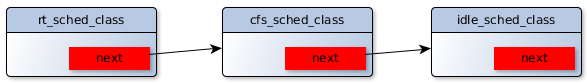
\includegraphics[width=\textwidth]{images/sched_classes}
        \caption{Scheduling classes in Linux}
        \label{fig:sched_classes}
\end{figure}
The basic scheduling unit in Linux is the \emph{scheduling entity},
which represents both tasks and task groups. There are two kinds of
scheduling entities \footnote{Both are defined in
  include/linux/sched.h}: CFS (scheduling) entities and RT
(scheduling) entities.  They are separately defined by \texttt{struct
  sched\_entity} and \texttt{struct sched\_rt\_entity}.  When we say a
task is enqueued in a runqueue, more precisely, it is the task's (CFS
or RT) scheduling entity that is enqueued.
\begin{lstlisting}[language=C, 
			caption={\texttt{A task embeds scheduling entities}},
			label={task_struct}]
struct task_struct {
	...
	struct sched_entity se;
	struct sched_rt_entity rt;
	...
};
\end{lstlisting}
Both CFS and RT entities are embedded in \texttt{struct task\_struct}. 
For any task, its status can switch between a CFS task and a RT task
through the system call \texttt{sched\_setscheduler}.

When \texttt{CONFIG\_FAIR\_GROUP\_SCHED} is set, CFS task grouping is
enabled. And \texttt{CONFIG\_RT\_GROUP\_SCHEED} is the kernel
configuration for RT task group scheduling. A task group can contains
both RT tasks and normal tasks, as shown in listing
\ref{task_group}. For each CPU, a task group uses a RT entity and a
CFS entity to represent its RT tasks and normal tasks.  Each type of
tasks inside a task group is scheduled independently by its own
scheduling class.
\begin{lstlisting}[language=C,
			caption={\texttt{A task group}},
			label={task_group}]		

struct task_group {
#ifdef CONFIG_FAIR_GROUP_SCHED
	/* sched_entity of this group on each cpu */
	struct sched_entity **se;
	...
#endif
#ifdef CONFIG_RT_GROUP_SCHED
	/* sched_rt_entity of this group on each cpu */
	struct sched_entity **rt_se;
	...
#endif
	...
};
\end{lstlisting}

\subsection{Runqueue centered scheduling\label{LinuxSched_rq}}

Every hook in \texttt{struct sched\_class} deals with the data
structure \texttt{struct rq}\footnote{Defined in kernel/sched/core.c},
which is called runqueue in Linux.  We say that Linux scheduling is
runqueue centered. In Linux, the \texttt{struct rq} is a per CPU data
structure; each cpu is associated with a runqueue. Despite its name,
\texttt{struct rq} is not a queue. The \texttt{struct rq} contains a
large amount of information. Its partial contents that are necessary
for understanding the remaining of the thesis are listed below.
\begin{lstlisting}[language=C,
			caption={\texttt{The runqueue structure}},
			label={runqueue}]
struct rq {
	...
	unsigned long nr_running;
	struct cfs_rq cfs;
	struct rt_rq rt;
	struct task_struct *curr, *idle;
	u64 clock;
	u64 clock_task;
#ifdef CONFIG_SMP
	int cpu;
#endif
	...
};
\end{lstlisting}
\begin{itemize}
\item \texttt{nr\_running} specifies the number of runnable tasks 
	having been enqueued in the runqueue.
\item \texttt{cfs and rt} are two specific runqueues for 
	\texttt{cfs\_sched\_class} and \texttt{rt\_sched\_class} respectively. 
	In order to handle specific type of tasks, different schedulers define 
	new type of runqueue data structures. 
	When we say a task is enqueued into a runqueue, it is finally into
	its corresponding specific runqueue.Each task group has one CFS 
	runqueue and RT runqueue per CPU to enqueue the tasks and sub task
	groups it contains in that CPU. 
	Figure \ref{task_group1} adds this new information to the
	knowledge just introduced for a task group, as in 
	figure \ref{task_group}. The default task group in the system points
	their CFS runqueue and RT runqueue to fields contained in the
	per CPU runqueue directly. 
\item \texttt{curr} points to the task currently running in this runqueue.
\item \texttt{idle} points to a special idle task. This is the task occupying
		the CPU  when no other tasks are runnable.
\item \texttt{clock and clock\_task} are time information kept by the runqueue.
	They updated by \texttt{update\_rq\_clock} method and some scheduling
	operation can rely them as time source.
\item \texttt{cpu} tells the CPU of this runqueue.
\end{itemize}
\begin{lstlisting}[language=C,
caption={\texttt{Specific runqueue information within a task group}},
			label={task_group1}]		

struct task_group {
#ifdef CONFIG_FAIR_GROUP_SCHED
	/* sched_entity of this group on each cpu */
	struct sched_entity **se;
	/* runqueue "owned" by this group on each cpu */
	struct cfs_rq **cfs_rq;
	...
#endif
#ifdef CONFIG_RT_GROUP_SCHED
	/* sched_rt_entity of this group on each cpu */
	struct sched_entity **rt_se;
	struct rt_rq **rt_rq;
	...
#endif
	...
};
\end{lstlisting}

\subsection{Completely Fair scheduler\label{sec:LinuxSched_cfs}}

The Completely Fair Scheduler (CFS) is implemented in
\texttt{fair\_sched\_class}.  Most tasks inside Linux are scheduled by
completely fair scheduling class and are normal tasks, which can be
further divided into three sub types given scheduling policies
(\texttt{SCHED\_NORMAL}, \texttt{SCHED\_BATCH} and
\texttt{SCHED\_IDLE\footnote{This SCHED\_IDLE policy is not related to
    idle\_sched\_class which aims to handle a special idle task.}}).

CFS tries to distribute CPU cycles fairly to tasks and task groups
according to their \emph{weight}. A specific runqueue structure
\texttt{struct cfs\_rq} is provided to deal with normal tasks.  Recall
that an instance of such cfs runqueue is embedded in the per-CPU
runqueue and each task group holds a pointer to cfs runqueue on each
CPU to store CFS tasks belonging to it.  A little more details on CFS
runqueue and CFS scheduling entity follow.
%The scheduling entity handled by CFS scheduling class is 
%\texttt{struct sched\_entity}. Here instead of studying the details of
%CFS, we are going to see how different scheduling components
\begin{lstlisting}[language=C,
		caption={\texttt{The CFS runqueue}},
		label={cfsrunqueue}]
struct cfs_rq {
        unsigned long nr_running;
        struct rb_root tasks_timeline;
#ifdef CONFIG_FAIR_GROUP_SCHED
        struct rq *rq;  
	struct task_group *tg;
#endif
	...
};
\end{lstlisting}
\begin{itemize}
\item \texttt{nr\_running} is the number of CFS tasks(entities) in this CFS 
	runqueue.
\item \texttt{tasks\_timeline} is the root of the red-black tree 
	\cite{rbtree} where 
	all CFS entities enququed into this CFS runqueue is stored. 
	This article will not go into details of the red-black tree
	mechanism, people only need to know it is an efficient way 
	to sort and access data elements.
\item \texttt{rq} is the per CPU runqueue that the task group \texttt{tg} 
	is finally enqueued.
\item \texttt{tg} is the task group that owns this CFS runqueue.
\end{itemize}
\begin{lstlisting}[language=C,
			caption={\texttt{The CFS scheduling entity}},
			label={sched_entity}]
struct sched_entity {
	...
	struct cfs_rq *cfs_rq;
#ifdef CONFIG_FAIR_GROUP_SCHED
	struct cfs_rq *my_q;
#endif
	...
}; 
\end{lstlisting}
\begin{itemize}
\item \texttt{cfs\_rq} is where this entity is to be queued.
		
\item \texttt{my\_rq} is the CFS runqueue owned by this entity(group).
	Remember that a scheduling entity can also represent a task group.
\end{itemize}
Now there is enough information to show how different scheduling components
(\texttt{sched\_entity}, \texttt{task\_struct}, \texttt{task\_group}
and \texttt{struct cfs\_rq}) are related in completely fair scheduler.

In this case that CFS task group scheduling is enabled. The CFS
scheduling scheme is shown in figure\ref{fig:cfs_scheme_tg}.  This is
not a complete scheme: 

\begin{enumerate}
\item Under a task group there could be sub groups, which behave as
  the task in the figure 
\item In the system, there is a top group, which includes all tasks in
  the system by default; tasks in this group are enqueued in the CFS
  runqueue embedded in the per CPU runqueue directly.
\end{enumerate}
\begin{figure}[htbp]
        \centering
        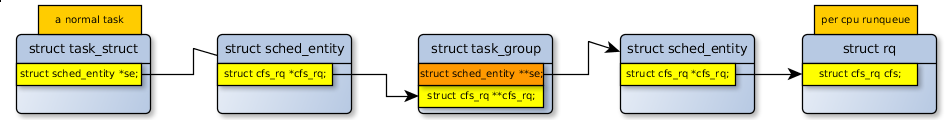
\includegraphics[width=\textwidth]{images/cfs_scheduling_scheme_tg}
        \caption{CFS scheduling when CFS group scheduling is enabled.}
        \label{fig:cfs_scheme_tg}
\end{figure}

If CFS task group scheduling is not enabled, a task is directed to its
per CPU runqueue by a \emph{task\_rq} marco. \emph{task\_rq} also
works for RT scheduling when RT task group scheduling is not enabled.
In fact, this \texttt{task\_rq} can be used even in case RT and CFS
task group scheduling are enabled. It just that when such task group
schedling are set, normally the information in each element in the
scheduling route is more important than simply returning a runqueue.
%\ref{fig:cfs_scheme_no_tg}.
\begin{figure}[htbp]
        \centering
        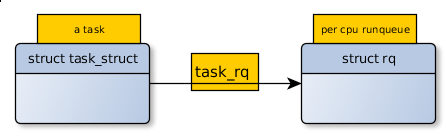
\includegraphics[height=0.1\textheight,width=0.5\textwidth]{images/scheduling_scheme_no_tg}
        \caption{Scheduling scheme without group scheduling}
        \label{fig:cfs_scheme_no_tg}
\end{figure}

We call the scheme in Figure \ref{fig:cfs_scheme_tg} and
\ref{fig:cfs_scheme_no_tg} \emph{scheduling routes} in CFS scheduling.
The route source is a task and the destination is a runqueue.  The
feature of a scheduling route is that if one component in the route is
known, then other scheduling components in the direction towards the
destination can be tracked.  The concept of scheduling route is first
invented in our work.  Later you will see the theory behind oxc
framework explores scheduling routes in Linux extensivly. We believe a
new concept is deserved in formalizing the work for oxc framework.

\subsection{Real time scheduler\label{sec:LinuxSched_rt}}

Tasks with POSIX real time policies \texttt{SCHED\_FIFO} and \texttt{SCHED\_RR}
are scheduled by the real time scheduling class \texttt{rt\_sched\_class} and
are called RT tasks. Given figure\ref{fig:sched_classes}, RT tasks are always
schedueld over normal tasks. 

\texttt{SCHED\_FIFO} implements a simple first-in, first-out scheduling 
algorithm. A running \texttt{SCHED\_FIFO} task can only be preempted by a 
higher priority RT task. \texttt{SCHED\_RR} is \texttt{SCHED\_FIFO} with 
timeslices --- it is a round robin algrithm. When a \texttt{SCHED\_RR}
task exhausts its timeslice, another \texttt{SCHED\_RR} task of the same
priprity is picked to run a timeslice, and so on. In either case, a RT task
cannot be preempted by a lower priority task.

The RT scheduling class provides with a sub runqueue structure 
\texttt{struct rt\_rq} to deal with RT tasks.
\begin{lstlisting}[language=C,
		caption={\texttt{The RT runqueue}},
		label={rtrunqueue}]
struct rt_rq {
	struct rt_prio_array active;
        unsigned long rt_nr_running;
#ifdef CONFIG_RT_GROUP_SCHED
        struct rq *rq;
        struct task_group *tg;
#endif
	...
};

struct rt_prio_array {
	DECLARE_BITMAP(bitmap, MAX_RT_PRIO+1); 
	struct list_head queue[MAX_RT_PRIO];
};
\end{lstlisting}
All RT tasks with the same priority, let's say $prio$, are kept in a linked 
list headed by $active.queue[prio]$. If there is a task in the list, the 
corresponding bit in $active.bitmap$ is set. All other fields have the same
meaning as in CFS runqueue. Compare with the CFS scheduling entity, the 
following \texttt{struct sched\_rt\_entity} is self explanatory enough. 
\begin{lstlisting}[language=C,
		caption={\texttt{The RT scheduling entity}},
		label={rt_entity}]
struct sched_rt_entity {
	...
	struct rt_rq *rt_rq;
#ifdef CONFIG_RT_GROUP_SCHED
	struct rt_rq *my_q;
#endif
	...
}; 
\end{lstlisting}

%The connections among \texttt{struct sched\_rt\_entity} and other scheduling
%components are similar to the \text{struct sched\_entity} case.
When \texttt{CONFIG\_RT\_GROUP\_SCHED} is set, figure\ref{fig:rt_scheme_tg} 
shows the scheduling route for RT scheduling. If RT task group scheduling is 
not enabled, still \emph{task\_rq} marco will be used.
\begin{figure}[htbp]
        \centering
        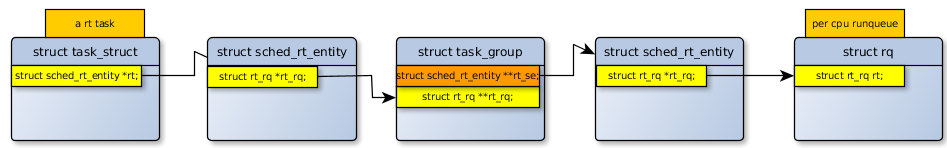
\includegraphics[width=\textwidth]{images/rt_scheduling_scheme_tg}
        \caption{RT scheduling when RT group scheduling is enabled.}
        \label{fig:rt_scheme_tg}
\end{figure}

\section{Related work\label{sec:RelatedWork}}
\subsection{RT throttling\label{sec:RelatedWork_RT}}
Enabling \texttt{CONFIG\_RT\_GROUP\_SCHED} lets users explicitly allocate
CPU bandiwidth to RT tasks in task groups. It uses the \emph{control group}
(cgroup) virtual file system. Each cgroup associates a set of tasks with
a set of resources, called \emph{subsystems}. For example \emph{cpuset} 
subsystem is responsible for assigning a set of CPUs and Memory Nodes to
tasks in a cgroup. Such tasks and resources can be further distributed in 
sub cgroups. Each cgroup is represented by a directory in the cgroup file 
system and a hierarchy of cgroups maps to a hierarchy of directories. In 
the directory, each mounted subsystem provides a list of files that are used 
as interfaces to control the allocation of a resource.
Through mounting the \emph{cpu} subsystem, two interfaces $cpu.rt\_period\_us$ 
and $cpu.rt\_runtime\_us$ are used to control the CPU bandwidth for RT 
tasks in each cgroup. That is, the total execution time of RT tasks in a cgroup 
on each CPU in time length $rt\_period\_us$ cannot exceed $rt\_runtime\_us$. 
If this constraint is met, RT tasks would not be choosen to run on that CPU 
until a new period; we call such tasks be throttled.

No matter \texttt{CONFIG\_RT\_GROUP\_SCHED} is set or not, in order to avoid RT 
tasks forever occupy thc CPU, there is a system wide setting that constraints
rt tasks' execution through the /proc virtual file system :

	$/proc/sys/kernel/sched\_rt\_period\_us$ 

	$/proc/sys/kernel/sched\_rt\_runtime\_us$ 
\\This applies to all RT tasks in a system.

\subsection{CFS bandwidth control\label{RelatedWork_CFS}}
Basically, CFS bandwidth control is the same technique as RT throttling
applying on normal tasks. It is a \texttt{CONFIG\_FAIR\_GROUP\_SCHED} 
extension which allows the specification of the maximum CPU bandwidth
available to normal tasks  in a cgroup or cgroup hierarchy.
The bandwidth allowed to a cgroup is specified using a 
quota(\texttt{cpu.cfs\_quota\_us}) and a period(\texttt{cpu.cfs\_period\_us}).
By specifying this, normal tasks in a cgroup will be limited to 
\texttt{cfs\_quota\_us} units of CPU time within the period of 
\texttt{cfs\_period\_us}. Recall that in RT throttling \ref{sec:RelatedWork_RT},
the reserved bandwidth through cgroup interfaces are applied in each CPU
individually.
\subsection{AQuoSA\label{sec:AQuoSA}}
The Adaptive Quality of Service Architecture composes two parts: 
a resource reservation scheduler an a feedback-based
control mechanism. The scheduler uses CBS rules to rserve CPU bandwidth for
a task, which is a RT task with SCHED\_RR policy in its Linux implementation.
Given the error between the reserved computation and the amount of CPU cycles
really consumed, the feedback controller adapts CBS reservation paramters to
provide quality of service CPU allocation in the system.
The control mechanism depends on CBS performance, not the scheduling details.
That is, such a control mechanism can be applied to general CBS based 
scheduling. AQuoSA lacks considerations on multi-processor platform.
  
\subsection{Schedule-deadline patch}
The schedule-deadline patch for Linux kernel is being developed to extend
current mainline Linux with a deadline-based scheduling method. 
In schedule-deadline, a new scheduling class (scheduler) is implemented and 
has highest priority among all scheduling classes. Tasks scheduled by this
scheduling class are called sched tasks. A sched task is assigned deadlines
according to CBS rules and scheduled in ''earliest deadline first (EDF)'' way.
\subsection{IRMOS real-time framework}
The rague name IRMOS comes from the European project ''Interactive Real-time
Multimedia Applications on Service Oriented Infrastructures''. 
The IRMOS 
framework replace RT throttling mechanism in mainline Linux with real time
CPU reservation(still CBS), and reuses the existing interfaces. So, users 
configure the cgroup interface as what we saw in RT 
throttling(\ref{sec:RelatedWork_RT}), the difference is that this time the CPU 
bandwidth is allocated in a guaranteed way. Also, new cgroup interfaces are 
added to assist reserved CPU power distribution in the cgroup hierarchy.

%%% Local Variables: 
%%% mode: latex
%%% TeX-master: "main"
%%% End: 

\chapter{Design and development\label{chap:design}}

\section{Open-Extension Container Structure\label{sec:design_oxc}}


Linux scheduling is runqueue, \texttt{struct rq}, centered and each 
scheduling class 
implements a set of interfaces to deal with the runqueue structure.
In mainline Linux, \texttt{struct rq} is a per CPU structure.
Each scheduling class defines its scheduling operations (enqueue, 
dequeue, etc.) with this per CPU runqueue. On Multiple processor
platform, tasks can migrate between different runqueues, also depending
on behaviours defined in specific scheduler.
In other words, on each CPU, a scheduling system is built up bsed on the
associated runqueue.
Different per CPU scheduling systems cooperate
with each other by task migrations defiend by specific scheduling class 
and construct the system level scheduling. 
The idea is that if there is one extra runqueue, each scheduler can still 
use it as scheduling parameter and a scheduling system can be built around 
it. If there are more than one extra runqueues, they can produce a pseudo 
system level scheduling system.   

Here a data structure named Open-Extension Container(OXC) is proposed,
shown in figure\ref{fig:oxc}.
\begin{figure}[htbp]
        \centering
        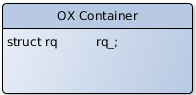
\includegraphics[width=0.5\textwidth]{images/oxc}
        \caption{Open-Extension Container}
        \label{fig:oxc}
\end{figure}
The ox container is designed as an abstract data structure; that is, any data
structure contains a \texttt{struct rq} runqueue inside can be called an ox
container. Now, in the system there is not only per CPU runqueues, but also 
per oxc runqueues.

\section{The oxc scheduling\label{sec:design_oxc_scheduling}}
As ox containers are defined, there are extra runqueues besides per CPU ones 
in a system. For each scheduler, they manage tasks above runqueues according
to implementation details in their scheduling class, and as long as a runqueue
parameter is provided for their schedulinf operations, they have do not care 
it is from a CPU or an ox container.
So as a oxc local runqueue is passed to hooks of scheduling classes, tasks would 
enqueue, operate and dequeue on a per container runqueue. As for tasks and scheduling
classes, there is no difference between a per CPU and per container runqueue.
This can be clearly shown when we see the scheduling scheme in the system 
with oxc scheduling. Recall the path which relates each
task with the per CPU runqueue it runs above in section \ref{sec:LinuxSched_cfs}
and \ref{sec:LinuxSched_rt}. Now let's see the scheduling scheme after the 
ox container joins the system with its local runqueue. 

From figure \ref{fig:oxc_fair_tg} and \ref{fig:oxc_rt_tg} we can see when 
task group scheduling is enabled, the scheduling route we saw before can also
lead a task to its per container runqueue. The same codes can still be used to
find both kinds of runqueues.

\begin{figure}[htbp]
	\begin{subfigure}
        \centering
        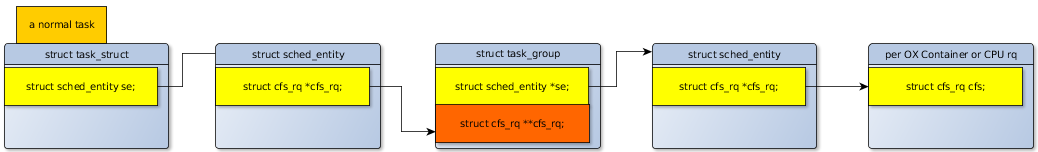
\includegraphics[height=2.5cm, width=\textwidth]{images/cfs_scheduling_scheme_tg_oxc}
        \caption{cfs}
        \label{fig:oxc_fair_tg}
	\end{subfigure}
	
	\begin{subfigure}
        \centering
        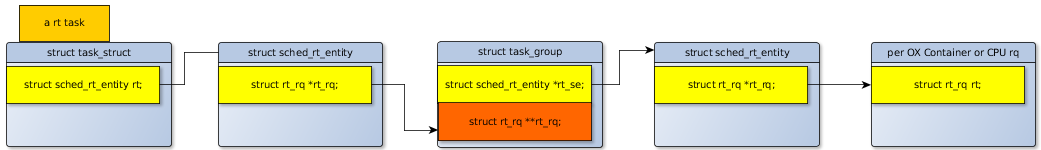
\includegraphics[height=2.5cm, width=\textwidth]{images/rt_scheduling_scheme_tg_oxc}
        %\caption{RT task group shceduling is enabled}
        \label{fig:oxc_rt_tg}
	\end{subfigure}
	\caption{Scheduling route with task group scheduling 
						in OXC enabled Linux}
	\label{fig:scheduling_route_oxc}
\end{figure}

In section \ref{sec:LinuxSched_cfs}, we introduce that when task group
scheduling is not enabled, a macro \texttt{task\_rq} is used to associate
a task to its runqueue. The \texttt{task\_rq} is defined as follows:
\begin{lstlisting}
#define task_rq(p)              cpu_rq(task_cpu(p))
\end{lstlisting}
The macro returns the associated rq for the CPU where the task is currently 
running on. So, when task group scheduling is not enabled, in order to merge
oxc scheduling in the system, a new route to lead a task to a runqueue is 
needed, shown in figure \ref{fig:oxc_task_no_tg}. Actually, this path already 
exists in Linux kernel. Just because in current Linux, there is no runqueue 
other than per CPU ones and people ignore to exploit it.  
\begin{figure}[htbp]
        \centering
        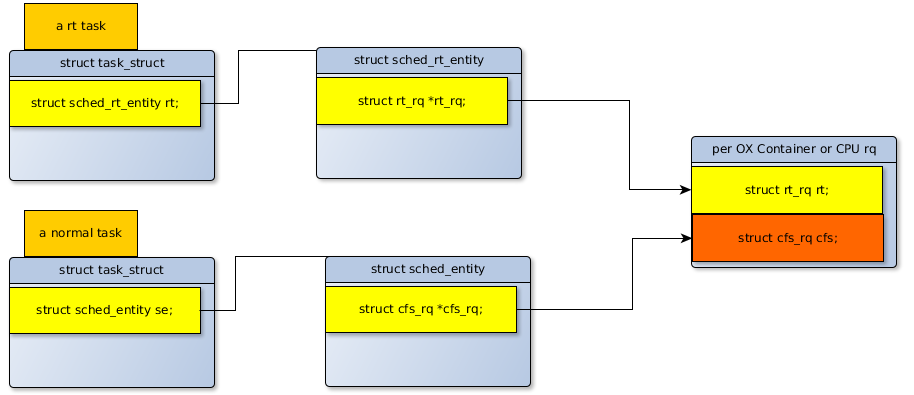
\includegraphics[width=\textwidth]{images/oxc_task_no_tg}
        \caption{New scheduling route for tasks when task group scheduling is not enabled}
        \label{fig:oxc_task_no_tg}
\end{figure}

The first feature of oxc scheduling is that it is compatibe with Linux original
scheduling. Tasks dealt by rt scheduler or cfs can naturally work under the
oxc scheduling system. When there is new scheduling algorithm implemented in
Linux kernel, like the \emph{sched deadline} patch we mentioned before, the
new scheduler has to fullfill details behind scheduling interfaces in 
\texttt{struct sched\_class}. Again, for each shceduling class, they do not
care the interface is passed a per CPU or per container runqueue as the
parameter, and the new scheduling class can also work under oxc scheduling.
So, the ox container structure is open to extension; this is where the name
is from.

Based on per CPU scheduling, each scheduling operation defined in 
\texttt{struct sched\_class} will affect all tasks in the CPU. The
oxc scheduling provides another opportunity to apply a scheduling class in a 
fine grained scale. Now, the scale to apply a scheduler can be controlled 
in the unit of an ox container. 

\section{Movtivation for oxc scheduling framework}
In section \ref{sec:RelatedWork}, we see that based on Linux CPU bandwidth 
control can be applied in the level of single tasks or task groups which 
are shceudled by some policies. Such control can be real-time or non real-time.
One obervation here is that there does not exist a mechanism that can
control CPU bandwidth for all kinds of tasks as a whole.
Such a general control mechanism is the initial consideration of
OXC framework.

Suppose there is an ox container, different schedulers can use it to enqueue,
operate, and dequeue its tasks. If a fraction of CPU bandwidth can be assigned
to this oxc, all kinds of tasks will use it as running on a less powerful
machine. This is the oxc solution to realize CPU bandwidth control as a whole.


\section{Development of OXC scheduling framework}
The oxc framework is still ongoing. Stable codes can be found 
in github\footnote{https://github.com/YIYAYIYAYOUCHENG/linux}.
The oxc framework is not a scheduler, it only interests in CPU bandwidth
control to an oxc, which depends on modular schedulers to use it for 
scheduling tasks.

\subsection{Implementation of ox container structure}
An ox container \texttt{struct oxc\_rq} is implemented in Linux kernel.
An \texttt{struct oxc\_rq} can reserve bandwidth from a CPU using CBS
rules. The CPU reservation for oxc runqueue follows the implementation
of CBS reservation for a rt runqueue in IRMOS framework. 
In the following context, an \texttt{struct oxc\_rq} is also called ox 
container, container, and oxc runqueue for the same meaning. An oxc runqueue
also correspond to a constant bandwidth server in CBS theory. 
\begin{lstlisting}[language=C, caption={\texttt{struct oxc\_rq}},
                        label={oxc_rq}]
struct oxc_rq {
	unsigned long oxc_nr_running;
	inx oxc_throttled;
	u64 oxc_deadline;
	u64 oxc_time;
	u64 oxc_runtime;
	ktime_t oxc_period;
	struct hrtimer oxc_period_timer;
	raw_spin_lock oxc_runtime_lock;
	struct rq rq_;
	struct rq *rq;
	struct rb_node rb_node;
};
\end{lstlisting}

\begin{itemize}
\item \texttt{oxc\_nr\_running} is the number of tasks enqueued in the 
		container's local runqueue. We say these tasks work in 
		the ox container.
\item \texttt{oxc\_throttled} is set when an ox container runs out of
		its budget in a period.
\item \texttt{oxc\_deadline} is current deadline of this ox container,
		which is a server in CBS theory.
\item \texttt{oxc\_time} is currently consumed budget in a period.
\item \texttt{oxc\_runtime} and \texttt{oxc\_period} are CBS parameters:
		\texttt{oxc\_runtime} is maximum budget and 
		\texttt{oxc\_period} is the period.
\item \texttt{oxc\_period\_timer} is timer which will activate at recharging
		points. If at some point, the value of \texttt{oxc\_time} is 
		larger than the value of \texttt{oxc\_runtime}, then
		\texttt{oxc\_throttled} should be set until 
		\texttt{oxc\_period\_timer} fires to recharge the container.
\item \texttt{oxc\_runtime\_lock} guarantee that the timing information of the 
		oxc is updated in a consistant way.
\item \texttt{rq\_} is the local runqueue of the ox container.
\item \texttt{rq} points to a per CPU runqueue and this CPU is where the 
		ox container reserves bandwidth from.
\item \texttt{rb\_node} is used to put an ox quneueu in a red black tree.
		All oxc runqueues reserve bandwidth from the same CPU
		is put in a red black tree associated with this CPU.
		In this tree, an ox container's \texttt{oxc\_deadline} 
		value is used to order nodes.
		runqueue 
\end{itemize}

All oxc runqueues that reserve bandwidth from the same CPU are put in the 
same red black tree, which orders its nodes according to the ox container's
\texttt{oxc\_deadline} value. The one with latest deadline is stored in the
leftmost node. 
\begin{lstlisting}[language=C]
struct oxc_edf_tree {
	struct rb_root rb_root;
	struct rb_node *rb_leftmost;
};
\end{lstlisting}
The pointer \texttt{rb\_leftmost} helps fast access to the latest deadline
ox container in a CPU.

An ox container is responsible for reserving bandwidth from a CPU.
Th \texttt{struct hyper\_oxc\_rq} is defined to reserve bandwidth from
multiple CPUs. 
\begin{lstlisting}[language=C]
struct hyper_oxc_rq {
	cpumask_var_t cpus_allowed;
	struct oxc_rq ** oxc_rq;
};
\end{lstlisting}
\begin{itemize}
\item \texttt{cpus\_allowed} specifies the CPUs that are used to reserve 
				bandwidth.
\item \texttt{oxc\_rq} is an array of ox containers to reserve bandwidth 			
		from CPUs specified in \texttt{cpus\_allowed}.
\end{itemize}

\subsection{Extensions on original data structures}
Extensions are added in some original data structures in order to merge
newly defined data structures in the system. Such extensions are not complex.
\begin{lstlisting}[language=C, caption={Extensions in \texttt{struct rq}}]
struct rq {
	...
	int in_oxc;
	struct oxc_edf_tree oxc_edf_tree;
};
\end{lstlisting}
As the name says, for an ox container's local runqueue, its 
\texttt{in\_oxc} field is set. And \texttt{oxc\_edf\_tree} in a 
per CPU runqueue help locate the ox container's edf tree in a CPU.

In current implementation of oxc framework, reservation is made for 
tasks in a control group. Tasks in a cgroup is represented in the
\texttt{struct task\_group} structure. So extensions also happen inside it.
\begin{lstlisting}[language=C, caption={Extensions in 
						\texttt{struct task\_group}}]
struct task_group {
	...
	struct hyper_oxc_rq *hyper_oxc_rq;
	int oxc_label;
};
\end{lstlisting}
Because tasks in a group can span multiple CPUs, the hyper container is
used to reserve bandwidth for it.
If a task group runs above a hyper oxc, its \texttt{hyper\_oxc\_rq} points 
to the hyper container; otherwise, this field is NULL.
When you associate a hyper container to a task group, its non oxc decendant 
task groups will also be associated with this hyper container, the 
\texttt{oxc\_label} field is used to specify this kind of sub task groups.

If a task runs in a ox container, it is called an oxc task. 
In section \ref{sec:design_oxc_scheduling}, we show how to direct a task
to the runqueue it runs above, which may be a per CPU or container one.
A further check of the runqueue's \texttt{in\_oxc} field can tell us
whether a task is an oxc task or not. Consider that such ''is that an oxc
task?'' is often used in the framework, a \texttt{is\_oxc\_task} field is
added in \texttt{struct task\_struct} for efficient reason.
\begin{lstlisting}[language=C, caption={\texttt{is\_oxc\_task} field in 
						\texttt{struct task\_struct}}]
struct task_struct {
	int is_oxc_task;
	...
};
\end{lstlisting}
When a task runs in an ox container, this field is set.

\subsection{The point to direct a task to a per ox container runqueue}
To schedule a task in a per oxc runqueue, the first thing is to associate
this task with the local runqueue of an oxc. To understand this, let's
first see how the system associate a task to a runqueue in mainline Linux,
where there is only per CPU runqueue concepts. 
\begin{lstlisting}[language=C, 
	caption={To associate a task with a runqueue in original Linux}]
void set_task_rq(struct task_struct *p, unsigned int cpu)
{
#ifdef CONFIG_FAIR_GROUP_SCHED
        p->se.cfs_rq = task_group(p)->cfs_rq[cpu];
        p->se.parent = task_group(p)->se[cpu];
#endif

#ifdef CONFIG_RT_GROUP_SCHED
        p->rt.rt_rq  = task_group(p)->rt_rq[cpu];
#endif
}
\end{lstlisting}
When task group scheduling is enabled, each task is directed to its task group.
This correspond to the first part of scheduling route. The second part of 
the scheduling route from task group to per CPU runqueue is done when the 
task group is created. Figure \ref{tg_creation} shows the hint how a 
task group joins the scheduling route during its creation.
\begin{figure}[htbp]
        \centering
        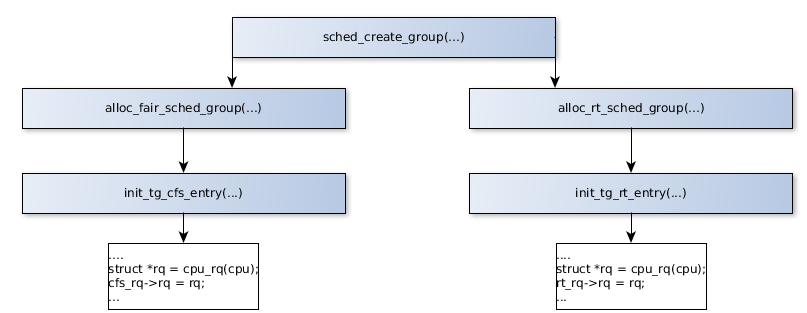
\includegraphics[width=\textwidth]{images/tg_creation}
        \caption{The creation of a task group in original Linux}
        \label{fig:tg_creation}
\end{figure}
In case that task group scheduling is not enabled, recall the scheduling path
where the \texttt{task\_rq} leads a task to its per CPU runqueue directly.

Now, we have seen the point a task joins the scheduling path in original Linux.
It's time to see the scenario after per oxc runqueue is imported in Linux.
Still, \texttt{set\_task\_rq} is the point to associate a task with a 
runqueue, per CPU or per oxc now.
\begin{lstlisting}[language=C, 
        caption={To associate a task with a runqueue under oxc framework}]
void set_task_rq(struct task_struct *p, unsigned int cpu)
{
        struct task_group *tg = task_group(p);

#ifdef CONFIG_FAIR_GROUP_SCHED
        p->se.cfs_rq = tg->cfs_rq[cpu];
        p->se.parent = tg->se[cpu];
#else
        if(!tg->hyper_oxc_rq)
                p->se.cfs_rq = &cpu_rq(cpu)->cfs;
        else
                p->se.cfs_rq = &tg->hyper_oxc_rq->oxc_rq[cpu]->rq_.cfs;
#endif

#ifdef CONFIG_RT_GROUP_SCHED
        p->rt.rt_rq  = tg->rt_rq[cpu];
        p->rt.parent = tg->rt_se[cpu];
#else
        if(!tg->hyper_oxc_rq)
                p->rt.rt_rq = &cpu_rq(cpu)->rt;
        else
                p->rt.rt_rq = &tg->hyper_oxc_rq->oxc_rq[cpu]->rq_.rt;
#endif
        if (task_rq_oxc(p)->in_oxc == 1)
                p->is_oxc_task = 100;
        else
                p->is_oxc_task = 0;
}
\end{lstlisting}
                                                  
When task group scheduling is enabled, there is no difference in cases of 
original Linux and oxc enabled Linux. The interesting part happens when 
task group scheduling is not set. This time, given the task group is associated
with a hyper oxc or not, the task is drected to a per CPU or oxc runqueue. This 
corresponds the scheduling route in figure \ref{fig:oxc_task_no_tg}. In 
the end of the method, \texttt{is\_oxc\_task} is configured. 
\texttt{task\_rq\_oxc} tracks the shceduling route to find the runqueue.

In oxc enabled Linux, a task group can be associated with a hyper oxc and
the runqueues it contains in three cases:1. when it is created, its parent is 
associated with a hyper oxc 2. the task group is explicitly attached to
a hyper oxc 3. one its acendant task group is attached to a hyper oxc.
\begin{figure}[htbp]
        \centering
        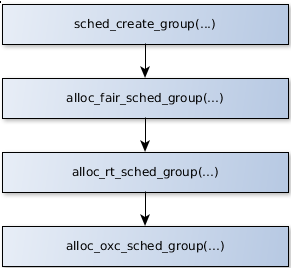
\includegraphics[height=0.25\textheight,width=0.5\textwidth]{images/tg_creation_oxc}
        \caption{The creation of a task group in oxc enabled Linux}
        \label{fig:tg_creation_oxc}
\end{figure}

\begin{lstlisting}[language=C,
        caption={OXC scheduling related initilization 
					during task group creation}]
int alloc_oxc_sched_group(struct task_group *tg, struct task_group *parent)
{
        int i;

        tg->hyper_oxc_rq = parent->hyper_oxc_rq;
        if( parent->hyper_oxc_rq) {
                for_each_possible_cpu(i) {
#ifdef CONFIG_FAIR_GROUP_SCHED
                        tg->cfs_rq[i]->rq =
                                &tg->hyper_oxc_rq->oxc_rq[i]->rq_;
                        if( !parent->se[i] && tg->se[i])
                                tg->se[i]->cfs_rq =
                                      &tg->hyper_oxc_rq->oxc_rq[i]->rq_.cfs;
#endif
#ifdef CONFIG_RT_GROUP_SCHED
                        tg->rt_rq[i]->rq =
                                &tg->hyper_oxc_rq->oxc_rq[i]->rq_;
                        if( !parent->rt_se[i] && tg->rt_se[i])
                                tg->rt_se[i]->rt_rq =
                                       &tg->hyper_oxc_rq->oxc_rq[i]->rq_.rt;
#endif
                }
                tg->oxc_label = 100;
        }
        else
                tg->oxc_label = 0;

        return 1;
}
\end{lstlisting}
\texttt{alloc\_oxc\_sched\_group} deals with oxc related initialization when a 
new task group is created. At first, the a newly created task group will inherit
its parent task group's hyper container. If the parent is an oxc task group, it
directs its scheduling path to the per oxc runqueue. And the \texttt{oxc\_label}
for such child oxc task group is 100.

A task group can direct to a OXC local runqueue explicitly through 
\texttt{init\_tg\_cfs\_entry\_oxc} and \texttt{init\_tg\_rt\_entry\_oxc}.
Let's have a look at \texttt{init\_tg\_cfs\_entry\_oxc} as an example.
\begin{lstlisting}[language=C, caption={To explicitlt direct a task group 
						to an OXC local runqueue}]
static void init_tg_cfs_entry_oxc(struct task_group *tg,
					struct cfs_rq *cfs_rq,
					struct sched_entity *se, int cpu,
					struct sched_entity *parent,
					struct oxc_rq *oxc_rq)
{
	struct rq *rq = rq_of_oxc_rq(oxc_rq);
	init_tg_cfs_entry(tg, cfs_rq, se, cpu, parent);
	tg->cfs_rq[cpu]->rq = rq;
	if( !parent && se)
		se->cfs_rq = &rq->cfs;
} 
\end{lstlisting}
Brief explaination on the parameters:
\begin{itemize}
\item \texttt{tg} is the task group to be dealt with.
\item \texttt{cfs\_rq} is the cfs runqueue the cfs entity of this task
		group is enqueued. 
\item \texttt{se} is the cfs entity that represents \texttt{tg}.
\item \texttt{cpu} specifies the cfs\_rq pointer inside \texttt{tg} that
		will be redirected.
\item \texttt{parent} points to the parent cfs scheduling entity.
\item \texttt{oxc\_rq} contains the destinated runqueue. 
\end{itemize}
As for codes, \texttt{rq\_of\_oxc\_rq} first returns the OXC local runqueue.
\texttt{init\_tg\_cfs\_entry} initialize CFS related work for \texttt{tg}.
Then, \texttt{tg} directs its local \texttt{cfs\_rq} for containing 
tasks on \texttt{cpu} to the per OXC runqueue just got. From now on, cfs 
tasks and task groups under \texttt{tg} work in the scheduling route which
will lead them to an OXC local runqueue. By directing a hierarchy of task
group to an OXC, there is a top group, which will be enqueud in the per
OXC runqueue's embedded cfs runqueue directly.

Now we see how to direct a task group to a per OXC runqueue when task group
scheduling is enabeld. In the whole procedure, tasks under this group is 
untouched.

\subsection{Run tasks under OXC scheduling framework}
As long as per OXC runqueue joins the scheduling route, the scheduling 
of tasks is compatible with modular schedulers in Linux. For an OXC task,
just pass the task itself and its OXC local runqueue, instead of per CPU
runqueue, to its corresponding scheduling class. And the scheduler will
behave as usual.

Because we consider reserving CPU bandwidth for an OXC runqueue, necessary
operations are performed before relaying a task to its modular scheduler.
Still scheduling details are not the framework's interest. 

In order to fullfill real time guarantee, oxc tasks are always privileged
to non oxc tasks. Amg oxc tasks inside a container, the priority relation
is the same as in Linux. The ox container itself can be considered as a 
virtual Linux system.

\subsubsection{To obtain the runqueue of a task}
A method \texttt{tas\_rq\_oxc} is used to obtain the runqueue of a task.
The runqueue retuned can be oxc local runqueue or per CPU one depending
that whether the task is inside a container.
\begin{lstlisting}[language=C]
struct rq* rq_of_task(struct task_struct *p)
{
	struct rq *rq;

#ifdef CONFIG_FAIR_GROUP_SCHED
	rq = p->se.cfs_rq->rq;
#else
	rq = task_rq_fair_oxc(p);
#endif
	return rq;
}
\end{lstlisting}
For any task, it has both cfs scheduling entity and rt entity. So the
rt and cfs scheduling routes both exists for a task. Here, we utilize
the cfs scheduling route. Given \texttt{CONFIG\_FAIR\_GROUP\_SCHED}
is set or not, the corresponding scheduling routes are explored to
track the runqueue.

\subsubsection{To enqueue an oxc task}
When an oxc task arrives, besides enqueue it in the oxc local runqueue,
the ox container information may be updated if necesary.
\begin{lstlisting}[language=C]
void enqueue_task_oxc(struct rq *rq, struct task_struct *p, int flags)
{
	struct oxc_rq *oxc_rq = oxc_rq_of_task(p);
	struct rq *rq_ = rq_of_oxc_rq(oxc_rq);

	/* Update the local runqueue' clock. */
	update_rq_clock(rq_);

	/*
	* Enqueue the task into the local runqueue
	* by its scheduling class.
	*/
	p->sched_class->enqueue_task(rq_, p, flags);

	inc_oxc_tasks(p, oxc_rq);
	enqueue_oxc_rq(oxc_rq);
}
\end{lstlisting}
\texttt{oxc\_rq\_of\_task} tracks the scheduling route and returns the ox
container of an oxc task. Then local runqueue's time information is updated.
Although the ox container does not care about scheduling details of tasks 
inside it, tasks are enqueued in its local runqueue and may rely the
runqueue's time information. Then we see all scheduling details are dealt 
by a task's scheduling class as the \texttt{enqueue\_task} of the
scheduling class is called with the task and local runqueue.
The \texttt{inc\_oxc\_tasks} method is simple.
\begin{lstlisting}[language=C]
static inline void inc_oxc_tasks(struct task_struct *p, struct oxc_rq *oxc_rq)
{
        oxc_rq->oxc_nr_running ++;
}
\end{lstlisting}

Until now, the oxc task has been put in the local runqueue. The coming of an
oxc task in a container may change the relation among ox containers in the
same edf tree. This is the work of \texttt{enqueue\_oxc\_rq} method. 
\begin{lstlisting}[language=C]
static void enqueue_oxc_rq(struct oxc_rq *oxc_rq)
{
        int on_rq;

        on_rq = oxc_rq_on_rq(oxc_rq);

        BUG_ON(!oxc_rq->oxc_nr_running);
        BUG_ON(on_rq && oxc_rq_throttled(oxc_rq));

        if( on_rq) {
                /* Already queued properly. */
                return;
        }
        /* We do not put a throttled oxc_rq in the edf tree. */
        if( oxc_rq_throttled(oxc_rq))
                return;

        oxc_rq_update_deadline(oxc_rq);
        __enqueue_oxc_rq(oxc_rq);
}
\end{lstlisting}
\texttt{on\_rq} tells if the container \texttt{oxc\_rq} is in a edf tree.
\texttt{BUG\_ON} is a Linux kernel macro. If the condition it checks is 
\texttt{true}, then the kernel will crash! Because we just put a task
in the local runqueue, so the first \texttt{BUG\_ON} should be passed.
When an ox container runs out of its budget, it should be moved from the
edf tree, this is what the second \texttt{BUG\_ON} checks. Now we pass
the two \texttt{BUG\_ONs}. If the \texttt{oxc\_rq} is already on edf 
tree or moved from the tree because of exhausting budget, nothing to
be done. There are two conditions for an ox container outside an edf
tree: it is throttled or it is empty. This means a task just joins
an empty container. Recall the CBS rules ''when a task arrives and 
the server is idle, update the deadline if necessary''. This is what
\texttt{oxc\_rq\_update\_deadline} does. When it comes to CPU reservation,
an ox container corresponds to a constant bandwidth server in CBS theory.
texttt{\_enqueue\_oxc\_rq} is quite a mechanical procesure to put an
oxc runqueue in an edf tree.

\subsubsection{To dequeue an oxc task}
\texttt{dequeue\_task\_oxc} is the opposite method of 
\texttt{enqueue\_oxc\_rq}.
\begin{lstlisting}[language=C]
static void dequeue_task_oxc(struct rq *rq, struct task_struct *p, int flags)
{
        struct rq *rq_ = task_rq_oxc(p);
        struct oxc_rq *oxc_rq = container_of(rq_, struct oxc_rq, rq_);

        /* Update the local runqueue. */
        update_rq_clock(rq_);
        /*
         * Dequeue the task from the local runqueue 
         * by its scheduling class.
         */
        p->sched_class->dequeue_task(rq_, p, flags);

        dec_oxc_tasks(p, oxc_rq);
        dequeue_oxc_rq(oxc_rq);
}
\end{lstlisting}
The structure of \texttt{dequeue\_task\_oxc} are the same as 
\texttt{enqueue\_task\_oxc}: local runqueue's time information is updated,
local runqueue and task is relayed to the corresponding scheduler, 
and the task number is decreased. When an oxc task leaves the container,
it is the time to check if the oxc is empty or not, which is done in
\texttt{dequeue\_oxc\_rq}.
\begin{lstlisting}[language=C]
static void dequeue_oxc_rq(struct oxc_rq *oxc_rq)
{
        int on_rq;

        on_rq = oxc_rq_on_rq(oxc_rq);
        /*
         * Here we do not expect throttled oxc_rq to be in the edf tree.
         * Note that when an oxc_rq exceeds its maximum budget,
         * it is dequeued via sched_oxc_rq_dequeue().
         */
        BUG_ON(on_rq && oxc_rq_throttled(oxc_rq));
        /* 
         * If an oxc_rq is not in the edf tree, it should be throttled or 
         * have no tasks enqueued.
         */
        BUG_ON(!on_rq && !oxc_rq_throttled(oxc_rq) && !oxc_rq->oxc_nr_running);

        if( on_rq && !oxc_rq->oxc_nr_running) {
                /* Dequeue the oxc_rq if it has no more tasks. */
                __dequeue_oxc_rq(oxc_rq);
                return;
        }
}
\end{lstlisting}
The comments are explainable enough. \texttt{\_\_dequeue\_oxc\_rq} removes 
a oxc runqueue from the edf tree.

\subsubsection{To check the preemption}
When a task wakes up from sleeping or is created, the scheduler will check 
if it can preempt current running task in the same CPU. If the current task
is an oxc task and the waking task is not an oxc task, the later cannot
preempt the current one. If both are non oxc tasks, Linux already has methods
to check. So here we only interest in the case when the waking task is an
oxc task.\\

\begin{lstlisting}[language=C]
static inline int
check_preempt_oxc_rq(struct task_struct *curr, struct task_struct *p, int flags)
{
        struct oxc_rq *oxc_rq = oxc_rq_of_task(p);
        struct oxc_rq *oxc_rq_curr = oxc_rq_of_task(curr);
        const struct sched_class *class;

	if(oxc_rq_throttled(oxc_rq)
		return 0;
        /* 
         * Tasks from a unthrottled oxc_rq always has a higher priority 
         * than non oxc tasks.
         */
        if( !oxc_rq_curr)
                return 1;

        /* Both p and current task are in the same oxc_rq. */
        if( oxc_rq_curr == oxc_rq) {
                if( p->sched_class == curr->sched_class) 
                        curr->sched_class->check_preempt_curr(
                                      &oxc_rq->rq_, p, flags);
                else {
                        for_each_class(class) {
                                if( class == curr->sched_class)
                                        break;
                                if( class == p->sched_class) {
                                        resched_task(curr);
                                        break;
                                }
                        }
                }

                return 0;
        }

        /* p and current tasks are oxc tasks from different ox containers. */
        return oxc_rq_before(oxc_rq, oxc_rq_curr);
}
\end{lstlisting}
\texttt{curr} and \texttt{p} are the current task and wakeing task respectively.
If task \texttt{p}'s container is throttled, it cannot preempt currently running task.
Otherwise, if \texttt{curr} is not an oxc task, \texttt{p} has higher priprity and
preempt \texttt{curr}. When two tasks are contained in the same oxc runqueue: if 
they are even in the same scheduling class, it's the modular scheduler's responsibility
to decide given; otherwise, the task whose scheduling class has higher priority in the
scheduler chain is chosen to run. In the last case, they two are from different 
containers. Now, \texttt{oxc\_rq\_before} checks if a contaienr's deadline is before
another's deadline. The one with smaller deadline will run. 

\subsubsection{To pick up an oxc task}
When to pick a most eligible task to run, oxc tasks should be checked first.
If there is no eligible oxc tasks, then non oxc tasks are considered.
\texttt{pick\_next\_task\_oxc} is responsible for choosing the most 
eligible oxc task in a CPU.
\begin{lstlisting}[language=C]
static struct task_struct* pick_next_task_oxc(struct rq *rq)
{
        struct oxc_rq *oxc_rq;
        struct rq *rq_;
        struct task_struct *p, *curr;
        const struct sched_class *class;
        /* This clock update is necessary! */
        update_rq_clock(rq);
        update_curr_oxc_rq(rq);
        oxc_rq = pick_next_oxc_rq(rq);
        if( !oxc_rq)
                return NULL;

        rq_ = rq_of_oxc_rq(oxc_rq);

        update_rq_clock(rq_);

        for_each_class(class) {
                if( class != &idle_sched_class) {
                        p = class->pick_next_task(rq_);
                        if( p) {
                                rq_->curr = p;
                                return p;
                        }
                }
        }

        return NULL;
}
\end{lstlisting}
There are one thing to note here: not only local runqueue's clock
is updated, but also the per CPU runqueue's clock is updated here.
This is because the reservation time of an ox container is counted
using the per CPU runqueue's clock and to keep the clock on time
for the container's use, here it is updated. 
\texttt{pick\_next\_oxc\_rq} picks the ox runqueue with latest 
deadline in a CPU. And along the scheduling class chain, each
scheduler uses its own way trying to find the most eligible
task in the local runqueue.
Another import method here is \texttt{update\_curr\_oxc\_rq}.
The budget comsumption really happens here.
\begin{lstlisting}[language=C]
static void update_curr_oxc_rq(struct rq *rq)
{
        struct task_struct *curr = rq->curr;
        struct oxc_rq *oxc_rq = oxc_rq_of_task(curr);
        u64 delta_exec;
        /*
         * If current task is not oxc task, simply return.
         */
        if( !oxc_rq)
                return;

        delta_exec = rq->clock - oxc_rq->oxc_start_time;
        oxc_rq->oxc_start_time = rq->clock;
        if( unlikely((s64)delta_exec < 0))
                delta_exec = 0;

        raw_spin_lock(&oxc_rq->oxc_runtime_lock);

        oxc_rq->oxc_time += delta_exec;
        if( sched_oxc_rq_runtime_exceeded(oxc_rq)) {
                resched_task(curr);
        }

        raw_spin_unlock(&oxc_rq->oxc_runtime_lock);
}
\end{lstlisting}
\texttt{update\_curr\_oxc\_rq} updates the runtime information of 
an oxc runqueue. If the budget in current period is exhausted, the
current task needs to be resched. the local spinlock 
\texttt{oxc\_runtime\_lock} protects the update of runtime from
interleave.
\begin{lstlisting}[language=C]
static int sched_oxc_rq_runtime_exceeded(struct oxc_rq *oxc_rq)
{
        u64 runtime = sched_oxc_rq_runtime(oxc_rq);
        u64 period = sched_oxc_rq_period(oxc_rq);

        /* 
         * If the runtime is set as 'RUNTIME_INF',
         * the ox container can run without throttling.
         */
        if( runtime == RUNTIME_INF)
                return 0;

        /* 
         * If the runtime to be larger the the period,
         * the ox container can run without throttling.
         */
        if( runtime >=period)
                return 0;

        /* There is still budget left. */
        if( oxc_rq->oxc_time < runtime)
                return 0;
        /* 
         * The reservation in a period has been exhausted,
         * to set the throttling label, remove the oxc_rq
         * from the edf tree and start the recharging timer.
         */
        else {
                oxc_rq->oxc_throttled = 1;
                sched_oxc_rq_dequeue(oxc_rq);
                start_oxc_period_timer(oxc_rq);

                return 1;
        }
}
\end{lstlisting}
Inside \texttt{sched\_oxc\_rq\_runtime\_exceeded}, at first
a series of non exceeded conditions are checked, which is 
easy to understand. The last \emph{else} statement deals with
the case tha tthe container is throttled: the \texttt{oxc\_throttled}
label is set, the oxc runqueue is removed from the edf tree and 
the timer is set and will fire at the next deadline to recharge the 
budget.

\chapter{Development of OXC Framework\label{chap:impl}}
The oxc framework is still ongoing. Latest codes can be found 
in github\footnote{https://github.com/YIYAYIYAYOUCHENG/linux}.
The oxc framework is not a scheduler. Although it cooperates with
different scheduling classes, its pure responsibility is managing 
the distribution of CPU power, which depends on modular schedulers 
to use it for scheduling tasks. Under oxc framework, we also call
oxc scheduling as oxc control since it is utilized to control CPU 
bandwidth reservation.

\section{Implementation of ox container structure}
An ox container \texttt{struct oxc\_rq}, listing~\ref{lst:oxc_rq}, 
is defined in Linux kernel. In \texttt{struct oxc\_rq} there 
are fields for reserving bandwidth from a CPU using CBS rules. 
In the following context, an \texttt{struct oxc\_rq} instance is 
also called an ox container, container, or oxc runqueue for the 
same meaning. An oxc runqueue also corresponds to a constant 
bandwidth server in CBS theory. 
The CPU reservation for oxc runqueues follows the implementation 
of CBS reservation for a RT runqueue in IRMOS framework. 

\begin{lstlisting}[language=C, caption={\texttt{struct oxc\_rq}},
                        label={lst:oxc_rq}]
struct oxc_rq {
	unsigned long oxc_nr_running;
	inx oxc_throttled;
	u64 oxc_deadline;
	u64 oxc_time;
	u64 oxc_runtime;
	ktime_t oxc_period;
	struct hrtimer oxc_period_timer;
	raw_spin_lock oxc_runtime_lock;
	struct rq rq_;
	struct rq *rq;
	struct rb_node rb_node;
};
\end{lstlisting}

\begin{itemize}
\item \texttt{oxc\_nr\_running} is the number of oxc tasks enqueued in 
		the container's local runqueue. We say these tasks work 
		in the ox container.
\item \texttt{oxc\_throttled} is set when an ox container runs out of
		its budget in a period.	Here ''throttled'' is a 
		convention inherited from RT throttling and 
		maps to the suspended state of a CBS. 
\item \texttt{oxc\_deadline} is current deadline of this ox container,
		which is a server in CBS theory.
\item \texttt{oxc\_time} is currently consumed budget in a period.
\item \texttt{oxc\_runtime} and \texttt{oxc\_period} are CBS parameters:
		\texttt{oxc\_runtime} is maximum budget and 
		\texttt{oxc\_period} is the period.
\item \texttt{oxc\_period\_timer} is timer which will activate at recharging
		time. If at some point, the value of \texttt{oxc\_time} is 
		larger than the value of \texttt{oxc\_runtime}, then
		the ox runqueue will be throttled and 
		its timer will be set to fire, at the 
		current deadline, \texttt{oxc\_deadline}, 
		to recharge the container.
\item \texttt{oxc\_runtime\_lock} guarantees that the update of an ox 
		container's reservation parameters (\texttt{oxc\_runtime} 
		and \texttt{oxc\_period}) and internal state 
		(\texttt{oxc\_time} and \texttt{oxc\_deadline}) happen
		in a consistant way.
\item \texttt{rq\_} is the local runqueue of the ox container.
\item \texttt{rq} points to a per CPU runqueue and its CPU is where the 
		ox container reserves bandwidth from.
\item \texttt{rb\_node} is used to put an ox runquneue in a red black tree.
		All oxc runqueues reserve bandwidth from the same CPU
		are sorted in a red-black tree. In this tree, an ox 
		container's \texttt{oxc\_deadline} value is used to order 
		nodes.
\end{itemize}
For each CPU, there is a red-black tree which stores all oxc runeueues that
reserve bandwidths in this CPU and orders them with their current deadline.
The oxc runqueue with earliest deadline is stored in the leftmost node. 
This tree is called the edf tree and is defined in 
\texttt{struct oxc\_edf\_tree}.

\begin{lstlisting}[language=C, caption={The EDF tree}]
struct oxc_edf_tree {
	struct rb_root rb_root;
	struct rb_node *rb_leftmost;
};
\end{lstlisting}
The pointer \texttt{rb\_leftmost} helps fast access to the earliest deadline
ox container in a CPU.

An ox container is responsible for reserving bandwidth from a CPU.
Another data structure \texttt{struct hyper\_oxc\_rq} is defined to 
reserve bandwidth from multiple CPUs. A \texttt{struct hyper\_oxc\_rq}
instance is called a hyper ox container. 

\begin{lstlisting}[language=C, caption={The hyper ox container}]
struct hyper_oxc_rq {
	cpumask_var_t cpus_allowed;
	struct oxc_rq ** oxc_rq;
};
\end{lstlisting}
\begin{itemize}
\item \texttt{cpus\_allowed} specifies the CPUs that are used to reserve 
				bandwidth.
\item \texttt{oxc\_rq} is an array of (pointers to) ox containers to 
		reserve bandwidth from CPUs identified in 
		\texttt{cpus\_allowed}.
\end{itemize}

\section{Extensions on original data structures\label{sec:extention}}
Several new data structures have been imported in the kernel that will
involve with Linux schedulers , yet the interfaces defined in 
\texttt{struct sched\_class} are kept unmodified. Extensions are added 
in some original data structures in order to merge newly defined data 
structures in the system. Such extensions are not complex.

\begin{lstlisting}[language=C, caption={Extensions on \texttt{struct rq}}]
struct rq {
	...
	int in_oxc;
	struct oxc_edf_tree oxc_edf_tree;
};
\end{lstlisting}
Two fileds are added in runqueue structure. The \texttt{in\_oxc} is 
used to distinguish per CPU and ox container runqueue.
As the name says, for an ox container's local runqueue, its 
\texttt{in\_oxc} field is set. And \texttt{oxc\_edf\_tree} in a 
per CPU runqueue is the edf tree for a CPU to keep and sort ox
containers.

The kernel configuration option \texttt{CONFIG\_CGROUP\_SCHED} is required
by the oxc framework. This option allows to create arbitrary task groups
using the "cgroup" pseudo filesystem. In current implementation of oxc 
framework, reservation is made for tasks in a control group. Tasks in a 
cgroup is represented in the \texttt{struct task\_group} structure. And 
extensions also happen inside it.

\begin{lstlisting}[language=C, 
			caption={Extensions on 
					\texttt{struct task\_group}}]
struct task_group {
	...
	struct hyper_oxc_rq *hyper_oxc_rq;
	int oxc_label;
};
\end{lstlisting}
Because tasks in a cgroup can span multiple CPUs, \texttt{struct task\_group}
is a good place to put the hyper ox container. If a task group has been
allocated CPU bandwidths through oxc control, then this task group runs 
inside a hyper ox container, and its \texttt{hyper\_oxc\_rq} points 
to that hyper container; otherwise, this field is NULL. As before,
a task group inside a hyper oxc is called an oxc task group.
There are three types of oxc task groups: an oxc group whose father
is not an oxc task group; an oxc task group whose father is an oxc group
with a different hyper ox container; an oxc task group with the same hyper
ox container as its father. The \texttt{oxc\_label} field is used to 
differ them. For non oxc task group, this field is not utilized.

When oxc scheduling is enabled in the kernel, there are two kinds of tasks
in the system: oxc tasks and non oxc tasks. To difference between them
is that oxc tasks work is (or will be) enqueued in an ox container's local 
runqueue and non oxc tasks work with a per CPU runqueue. So, from a task, 
its associated runqueue can be tracked according to the scheduling route 
in figure~\ref{fig:scheduling_route_oxc} or~\ref{fig:oxc_task_no_tg}.
As long as the runqueue is found, given its \texttt{in\_oxc} field, the 
status of this runqueue and the task can both be fixed. Consider that 
the question ''is that an oxc task?'' happens frequently in the framework, 
a \texttt{is\_oxc\_task} field is added in \texttt{struct task\_struct} for 
efficient recognition of an oxc task.

\begin{lstlisting}[language=C, caption={\texttt{is\_oxc\_task} field in 
						\texttt{struct task\_struct}}]
struct task_struct {
	int is_oxc_task;
	...
};
\end{lstlisting}
When a task runs in an ox container, this new field is set.

\section{To direct a task to a per ox container runqueue\label{sec:redir}}

In section~\ref{sec:design_oxc_scheduling}, we show the scheduling routes
when there exists oxc scheduling in a system. This section will introduce
the details on how to build these scheduling routes.

\subsection{To build the scheduling route in mainline Linux}

In order to schedule a task in a per oxc runqueue, the first thing is to 
associate this task with the local runqueue of an oxc. To understand this,
let's first see how the system associates a task to a runqueue in mainline 
Linux, where there is only per CPU runqueues. This is done through
the method \texttt{set\_task\_rq}.

\begin{lstlisting}[language=C, label={lst:set_task_rq},
	caption={To associate tasks with a per CPU runqueue in mainline Linux}]
void set_task_rq(struct task_struct *p, unsigned int cpu)
{
#ifdef CONFIG_FAIR_GROUP_SCHED
        p->se.cfs_rq = task_group(p)->cfs_rq[cpu];
        p->se.parent = task_group(p)->se[cpu];
#endif

#ifdef CONFIG_RT_GROUP_SCHED
        p->rt.rt_rq  = task_group(p)->rt_rq[cpu];
#endif
}
\end{lstlisting}

As demonstrated in list~\ref{lst:set_task_rq}, codes inside 
\texttt{set\_task\_rq} build up the front part of the scheduling route 
when \texttt{CONFIG\_FAIR\_GROUP\_SCHED} and 
\texttt{CONFIG\_RT\_GROUP\_SCHED} are set.
When RT or CFS task group scheduling is enabled, each task is then directed 
to its task group. In mainline Linux, the second part of a scheduling route
only directs a task group to the per CPU runqueues. Such paths are connected 
when the task group is created. Figure~\ref{fig:tg_creation} shows the hint how 
a task group joins the scheduling route during its creation. In addition, now 
we know that a scheduling route is built backwards from an runqueue end.

\begin{figure}[htbp]
        \centering
        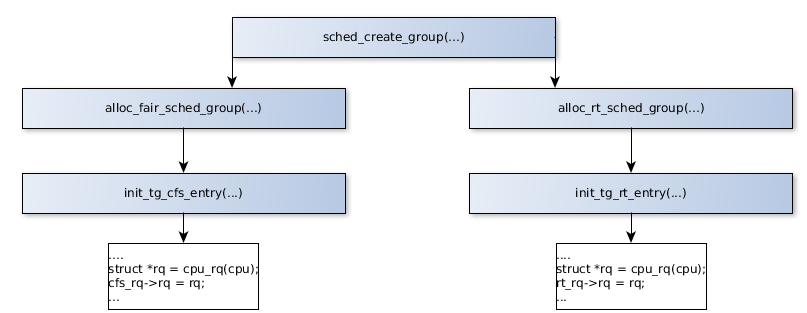
\includegraphics[width=\textwidth]{images/tg_creation}
        \caption{The creation of a task group in original Linux}
        \label{fig:tg_creation}
\end{figure}
In case that task group scheduling is not enabled, recall the scheduling path
where the \texttt{task\_rq} leads a task to its per CPU runqueue directly.

\subsection{To build the scheduling route in oxc enabled Linux}

Now, we have seen the point when a task or task group joins the scheduling 
route in mainline Linux. These points are still time to fill elements in 
scheduling routes, figure \ref{fig:scheduling_route_oxc} and 
\ref{fig:oxc_task_no_tg}, after oxc runqueues are imported in Linux.

Previously, the \texttt{set\_task\_rq} method does not deal with the task 
that is not in a RT or CFS task group. This is because for tasks without 
group scheduling, the scheduling route \texttt{task\_rq} is utilized.
However, \texttt{task\_rq} does not work for an oxc task to locate the
per container runqueue. The functionality of \texttt{set\_task\_rq} is
then extended to care about tasks without group scheduling. 

\begin{lstlisting}[language=C, 
        caption={The extended \texttt{set\_task\_rq}}]
void set_task_rq(struct task_struct *p, unsigned int cpu)
{
        struct task_group *tg = task_group(p);

#ifdef CONFIG_FAIR_GROUP_SCHED
        p->se.cfs_rq = tg->cfs_rq[cpu];
        p->se.parent = tg->se[cpu];
#else
        if(!tg->hyper_oxc_rq)
                p->se.cfs_rq = &cpu_rq(cpu)->cfs;
        else
                p->se.cfs_rq = &tg->hyper_oxc_rq->oxc_rq[cpu]->rq_.cfs;
#endif

#ifdef CONFIG_RT_GROUP_SCHED
        p->rt.rt_rq  = tg->rt_rq[cpu];
        p->rt.parent = tg->rt_se[cpu];
#else
        if(!tg->hyper_oxc_rq)
                p->rt.rt_rq = &cpu_rq(cpu)->rt;
        else
                p->rt.rt_rq = &tg->hyper_oxc_rq->oxc_rq[cpu]->rq_.rt;
#endif
        if (task_rq_oxc(p)->in_oxc == 1)
                p->is_oxc_task = 100;
        else
                p->is_oxc_task = 0;
}
\end{lstlisting}
                                                  
When task group scheduling is enabled, there is no difference for setting a 
task's runqueue in both
the mainline Linux and oxc enabled Linux. The interesting part happens when 
task group scheduling is not set. This time, given that the task group is 
associated with a hyper oxc or not, the task is drected to a per CPU runqueue
or per an oxc runqueue ( the container is supplied by the 
\texttt{hyper\_oxc\_rq}). This corresponds the first part of the scheduling 
route in figure~\ref{fig:oxc_task_no_tg}. In the end of the method, 
\texttt{is\_oxc\_task} label of a task is configured. When 
\texttt{task\_rq\_oxc} is invoked, the scheduling route for a task has already 
been set. It tracks the shceduling route to find the runqueue that a task is 
just associated. After this extended \texttt{set\_task\_rq} call, both routes 
with or without group scheduling are built up.

In the mainline Linux, the end part of a scheduling route is built up when
a task group is created. Within the oxc enabled kernel, things will be a 
little more complex. In the oxc applied Linux, a task group can be associated 
with a hyper oxc and the contained runqueues in three cases: 1) If its parent 
is associated with a hyper oxc, then when it is created it will inherit its 
parent's hyper ox container. 2) The task group is explicitly attached to
a hyper oxc. 3) When the group's one ascendant task group is attached to 
a hyper oxc, its \texttt{hyper\_oxc\_rq} field will point to that hyper 
oxc too. 

\begin{figure}[htbp]
        \centering
        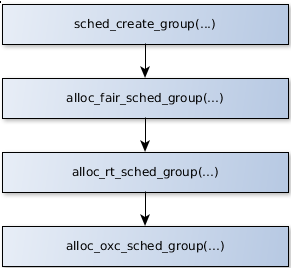
\includegraphics[height=0.25\textheight,width=0.5\textwidth]{images/tg_creation_oxc}
        \caption{The creation of a task group in oxc enabled Linux}
        \label{fig:tg_creation_oxc}
\end{figure}

Corresponding to case 1, now when a task group is created, there 
will be a initilization routine for oxc scheduling. A sketch is shown in 
figure \ref{fig:tg_creation_oxc}. The details of this routinue 
\texttt{alloc\_oxc\_sched\_group} is shown below. 

\begin{lstlisting}[language=C,
        caption={OXC scheduling related initilization 
					during task group creation}]
int alloc_oxc_sched_group(struct task_group *tg, struct task_group *parent)
{
        int i;

        tg->hyper_oxc_rq = parent->hyper_oxc_rq;
        if( parent->hyper_oxc_rq) {
                for_each_possible_cpu(i) {
#ifdef CONFIG_FAIR_GROUP_SCHED
                        tg->cfs_rq[i]->rq =
                                &tg->hyper_oxc_rq->oxc_rq[i]->rq_;
                        if( !parent->se[i] && tg->se[i])
                                tg->se[i]->cfs_rq =
                                      &tg->hyper_oxc_rq->oxc_rq[i]->rq_.cfs;
#endif
#ifdef CONFIG_RT_GROUP_SCHED
                        tg->rt_rq[i]->rq =
                                &tg->hyper_oxc_rq->oxc_rq[i]->rq_;
                        if( !parent->rt_se[i] && tg->rt_se[i])
                                tg->rt_se[i]->rt_rq =
                                       &tg->hyper_oxc_rq->oxc_rq[i]->rq_.rt;
#endif
                }
                tg->oxc_label = 100;
        }
        else
                tg->oxc_label = 0;

        return 1;
}
\end{lstlisting}

The \texttt{alloc\_oxc\_sched\_group} handles oxc related initialization when a 
new task group is created. At first, the a newly created task group will inherit
its parent task group's hyper container. If the parent is an oxc task group, 
this child task group will be directed to per oxc runqueues contained in the
hyper oxc; the result corresponds to the end part of a scheduling route.  
And the \texttt{oxc\_label} for such a child oxc task group is 100.

Case 2 and 3 actually happen at the same time. When explicitly putting the 
parent group inside a hyper ox container, the dscendant task groups will also 
be directed to this hyper oxc. Two methods \texttt{init\_tg\_cfs\_entry\_oxc} and
\texttt{init\_tg\_rt\_entry\_oxc} will be involved in this procedure to 
associate task groups with the hyper ox container. 
The structure in the two is silimar. As an example, Here we only study how the 
CFS part of a task group is handled through \texttt{init\_tg\_cfs\_entry\_oxc}.

\begin{lstlisting}[language=C, caption={To explicitly direct a task group 
						(CFS part) to an OXC \\
					\indent\hspace{5cm} local runqueue}]
static void init_tg_cfs_entry_oxc(struct task_group *tg,
					struct cfs_rq *cfs_rq,
					struct sched_entity *se, int cpu,
					struct sched_entity *parent,
					struct oxc_rq *oxc_rq)
{
	struct rq *rq = rq_of_oxc_rq(oxc_rq);
	init_tg_cfs_entry(tg, cfs_rq, se, cpu, parent);
	tg->cfs_rq[cpu]->rq = rq;
	if( !parent && se)
		se->cfs_rq = &rq->cfs;
} 
\end{lstlisting}
A brief explanation on the parameters:
\begin{itemize}
\item \texttt{tg} is the task group to be dealt with.
\item \texttt{cfs\_rq} is the CFS runqueue that this task group 
		owns. 
\item \texttt{se} is the CFS entity that represents \texttt{tg}.
\item \texttt{cpu} specifies the cfs\_rq pointer inside \texttt{tg} that
		will be redirected. The function 
		\texttt{init\_tg\_cfs\_entry\_oxc}
		redirects one CFS runqueue inside a \texttt{tg} to an oxc 
		runqueue, \texttt{oxc\_rq}, in each call. A hyper ox 
		container can have more than one oxc runqueues inside
		and \texttt{tg} has multiple CFS runqueues too.
		To relate a task group with a hyper ox container requires 
		the \texttt{init\_tg\_cfs\_entry\_oxc} be called multiple times.
\item \texttt{parent} points to the parent CFS scheduling entity.
\item \texttt{oxc\_rq} contains the destinated runqueue. 
\end{itemize}

As for codes, first \texttt{rq\_of\_oxc\_rq} returns the oxc local runqueue.
The mainline kernel method \texttt{init\_tg\_cfs\_entry} is then called to 
re-initialize CFS related work for \texttt{tg}. 
%This is a mainline Linux kernel function called in
%task group creation if CFS group scheduling is set.
The real bridging point is in the following line where 
\texttt{tg} connects its local \texttt{cfs\_rq} on 
\texttt{cpu} to the per oxc runqueue just got. After 
\texttt{init\_tg\_cfs\_entry\_oxc} is invoked over every CPU for the 
task group, CFS tasks and task groups under \texttt{tg} will work in 
the scheduling route leading them to an oxc local runqueue. When a task 
group is explicitly directed to a hyper ox container, the whole family of 
task groups under it will also be associated with this hyper ox container. 
This task group will be the top of this hierarchy, and it will be enqueued 
in the per oxc runqueue's embedded CFS runqueue directly. The last 
\texttt{if} condition returns true when \texttt{tg} is top in the oxc 
group hierarchy.
%One amazing feature of this procedure to relate a task group to a per oxc 
%runqueue is that it has nothing to do tasks under this group.

\section{Run tasks under OXC scheduling framework\label{sec:run}}

As long as per oxc runqueue joins the scheduling route, modular schedulers
can handle tasks in an ox container without differentiating oxc tasks from
non oxc tasks.
%the scheduling 
%of tasks is compatible with modular schedulers in Linux. 
In case to schedule an oxc task, just pass the task itself and its oxc 
local runqueue, instead of per CPU runqueue, to its corresponding 
scheduling class. The local runqueue of an oxc task can be easily tracked 
along the scheduling route. And the scheduler will behave as usual. That 
is, this oxc scheduling framework is transparent to both schedulers and 
tasks.

Because we consider reserving CPU bandwidth for an ox container, there
are scheduling operations that before or after passing parameters to them,
the reservation information should be updated. For these kinds of scheduling
operations, we adapt a relaying mechanism. The parameter is first passed to
another function and after necessary actions, the scheduling operation is
called inside this function. We say that such scheduling operations are
encapsulated in oxc (scheduling) functions.
Still scheduling details for a task are not the framework's work. 

In order to fulfil real time guarantee, oxc tasks are always privileged
to non oxc tasks. Among oxc tasks inside a container, the priority relation
is the same as in Linux. The ox container itself can be considered as a 
virtual Linux system.

For each scheduling operation defined in \texttt{struct sched\_class},
there are three fates for them under oxc scheduling framework: 
some are encapsulated inside oxc functions so as to work with oxc tasks; 
some can work under the framework directly; and others are not supported. 
The table~\ref{tab:op_classes} displays the three classes of scheduling 
operations. The naming convention for oxc functions which encapsulate 
a scheduling operation inside is appending the original name with 
\texttt{\_oxc}. For example, the scheduling operation
\texttt{task\_tick} is called inside in \texttt{task\_tick\_oxc}.
The enqueue and dequeue are two exceptions, they are enclosed in 
\texttt{enqueue\_task\_oxc} and \texttt{dequeue\_task\_oxc}.

\begin{table}[thbp]
  \centering
  \begin{tabular}{l|l|l}\hline
	\small{Work inside an oxc function} & \small{Work without encapsulation} & \small{Unsupported}\\\hline
		check\_preempt\_curr	& yield\_task				& Others	\\
		pick\_next\_task	& yield\_to\_task			&		\\
		put\_prev\_task		& task\_waking				&		\\
		set\_curr\_task		& task\_woken				&		\\
		task\_tick		& set\_cpus\_allowed			&		\\
		enqueue\_task\_rq	& task\_fork				&		\\
		dequeue\_task\_rq	& switched\_from			&		\\
					& switched\_to				&		\\
					& prio\_changed				&		\\
					& get\_rt\_interval			&		\\
					& task\_move\_group			&		\\\hline
  \end{tabular}	
  \caption{The way to handle a scheduling operation under the oxc framework}
  \label{tab:op_classes}
\end{table}

The following will be descriptions on oxc functions with emphasis on ones that
encapsulate a scheduling operation inside.

\subsection{To obtain the runqueue of a task\label{sec:rq_of_task}}
A method \texttt{rq\_of\_task}, listing~\ref{lst:rq_of_task}, is used to 
obtain the runqueue of a task. The runqueue retuned can be an oxc local 
runqueue or per CPU one depending that whether the task is inside a 
container. This function can be used to replace the \texttt{task\_rq} 
macro under oxc framework. For any task, it has both CFS scheduling 
entity and RT entity. And the RT and CFS scheduling routes both exists 
for a task. Here, we exploit the CFS scheduling route. Given 
\texttt{CONFIG\_FAIR\_GROUP\_SCHED} is set or not, the corresponding 
scheduling route is explored to track the runqueue.

\begin{lstlisting}[language=C, 
		caption={Codes to obtain the runqueue of a task},
			label={lst:rq_of_task}]
struct rq* rq_of_task(struct task_struct *p)
{
	struct rq *rq;

#ifdef CONFIG_FAIR_GROUP_SCHED
	rq = p->se.cfs_rq->rq;
#else
	rq = task_rq_fair_oxc(p);
#endif
	return rq;
}
\end{lstlisting}

One important use of this function is in \texttt{oxc\_rq\_of\_task}, 
which takes a task as the input, and returns the ox container the 
task is inside. In case the input is not an oxc task, 
\texttt{NULL} will be returned. The \texttt{oxc\_rq\_of\_task} is 
one most often invoked method under oxc framework. It first gets a 
task's runqueue using the \texttt{rq\_of\_task}, then obtains the ox 
container the runqueue is in, in case the runqueue is in an container.

\subsection{To enqueue an oxc task\label{sec:enqueue_task_oxc}}

When an oxc task arrives, besides enqueue it in the oxc local runqueue,
the ox container's reservation information may be updated if necesary.
The \texttt{enqueue\_task\_oxc} shows the typical scheme for oxc 
functions to enclose a scheduling operation.

\begin{lstlisting}[language=C, 
		caption={To enqueue an task into the oxc local runqueue}]
void enqueue_task_oxc(struct rq *rq, struct task_struct *p, int flags)
{
	struct oxc_rq *oxc_rq = oxc_rq_of_task(p);
	struct rq *rq_ = rq_of_oxc_rq(oxc_rq);

	/* Update the local runqueue' clock. */
	update_rq_clock(rq_);

	/*	
	* Enqueue the task into the local runqueue
	* by its scheduling class.
	*/
	p->sched_class->enqueue_task(rq_, p, flags);

	inc_oxc_tasks(p, oxc_rq);
	enqueue_oxc_rq(oxc_rq);
}
\end{lstlisting}

The method \texttt{oxc\_rq\_of\_task} tracks the scheduling route and 
returns the ox runqueue of an oxc task. Then the ox container's local 
runqueue's time information is updated. Although the ox container does 
not care about scheduling details of tasks inside it, tasks are indeed 
enqueued in its local runqueue and may rely the runqueue's time information. 
We can see that all scheduling details are carried out by a task's 
scheduling class as the \texttt{enqueue\_task} operation of the 
scheduling class is called with the task and local runqueue as inputs. 
The \texttt{inc\_oxc\_tasks} method simply increases the number of oxc 
tasks in the oxc runqueue by one. The reason that such a simple function 
is stiil kept is that as the framework grows more complex in the future, 
extra operations can be put in this method.

\begin{lstlisting}[language=C, 
		caption={To update the number of tasks inside a container} ]
static inline void inc_oxc_tasks(struct task_struct *p, struct oxc_rq *oxc_rq)
{
        oxc_rq->oxc_nr_running ++;
}
\end{lstlisting}

Until now, the oxc task has been put in the local runqueue. 
If before the arrival of this task the ox container is empty and not 
throttled, it is time to put this container in its EDF tree.
This is the work of \texttt{enqueue\_oxc\_rq} method. 

\begin{lstlisting}[language=C, 
		caption={To put an ox container in the EDF tree
					if necessary}]
static void enqueue_oxc_rq(struct oxc_rq *oxc_rq)
{
        int on_rq;

        on_rq = oxc_rq_on_rq(oxc_rq);

        BUG_ON(!oxc_rq->oxc_nr_running);
        BUG_ON(on_rq && oxc_rq_throttled(oxc_rq));

        if( on_rq) {
                /* Already queued properly. */
                return;
        }
        /* We do not put a throttled oxc_rq in the edf tree. */
        if( oxc_rq_throttled(oxc_rq))
                return;

        oxc_rq_update_deadline(oxc_rq);
        __enqueue_oxc_rq(oxc_rq);
}
\end{lstlisting}

\texttt{on\_rq} tells if the container \texttt{oxc\_rq} is in a edf tree.
\texttt{BUG\_ON} is a Linux kernel macro. If the condition it checks is 
\texttt{true}, then the kernel will crash! Because we just put a task
in the local runqueue, so the first \texttt{BUG\_ON} should be passed.
When an ox container runs out of its budget, it should be moved from the
edf tree, this is what the second \texttt{BUG\_ON} checks. Now we pass
the two \texttt{BUG\_ONs}. If the \texttt{oxc\_rq} is already on edf 
tree or moved from the tree because of exhausting budget, nothing needs 
to be done. There are two conditions for an ox container to be outside
an edf tree: it is throttled or it is empty. If the last \texttt{if}
condition is passed, this means a task just joins an empty container. 
Recall the CBS rules ''when a task arrives and the server is idle, update 
the deadline if necessary''. This is exactly what 
\texttt{oxc\_rq\_update\_deadline} does. When it comes to CPU reservation,
an ox container corresponds to a constant bandwidth server in CBS theory.
\texttt{\_enqueue\_oxc\_rq} is a quite mechanical procesure to put an
oxc runqueue in an edf tree.

\subsection{To dequeue an oxc task\label{sec:dequeue_task_oxc}}

\texttt{dequeue\_task\_oxc} is the opposite method of 
\texttt{enqueue\_oxc\_rq}.

\begin{lstlisting}[language=C, 
		caption={To remove a task from the oxc local runqueue}]
static void 
dequeue_task_oxc(struct rq *rq, struct task_struct*p, int flags)
{
        struct rq *rq_ = task_rq_oxc(p);
        struct oxc_rq *oxc_rq = container_of(rq_, struct oxc_rq, rq_);

        /* Update the local runqueue. */
        update_rq_clock(rq_);
        /*
         * Dequeue the task from the local runqueue 
         * by its scheduling class.
         */
        p->sched_class->dequeue_task(rq_, p, flags);

        dec_oxc_tasks(p, oxc_rq);
        dequeue_oxc_rq(oxc_rq);
}
\end{lstlisting}

The layout inside \texttt{dequeue\_task\_oxc} is the same as what we see in
\texttt{enqueue\_task\_oxc}: local runqueue's clock information is updated,
local runqueue and task are relayed to the corresponding scheduler, 
the task number and EDF tree are updated. When an oxc task leaves the 
container, it is the time to check if the oxc is empty or not, which is 
done in \texttt{dequeue\_oxc\_rq}.

\begin{lstlisting}[language=C,
		caption={To remove an ox container 
				from the EDF tree if necessary}]
static void dequeue_oxc_rq(struct oxc_rq *oxc_rq)
{
        int on_rq;

        on_rq = oxc_rq_on_rq(oxc_rq);
        /*
         * Here we do not expect throttled oxc_rq to be in the 
         * edf tree. Note that when an oxc_rq exceeds its 
         * maximum budget, it is dequeued via 
         * sched_oxc_rq_dequeue().
         */
        BUG_ON(on_rq && oxc_rq_throttled(oxc_rq));
        /* 
         * If an oxc_rq is not in the edf tree, it should 
         * be throttled or have no tasks enqueued.
         */
        BUG_ON(!on_rq && !oxc_rq_throttled(oxc_rq) && !oxc_rq->oxc_nr_running);

        if( on_rq && !oxc_rq->oxc_nr_running) {
                /* Dequeue the oxc_rq if it has no tasks. */
                __dequeue_oxc_rq(oxc_rq);
                return;
        }
}
\end{lstlisting}

The comments are explanable enough. \texttt{\_\_dequeue\_oxc\_rq} 
is the counterpart of \texttt{\_\_enqueue\_oxc\_rq} to remove an oxc
runqueue from the EDF tree.

\subsection{To check the preemption condition
			\label{sec:check_preempt_curr_oxc}}
When a task wakes up from sleeping or is created, the scheduler will check 
if it can preempt temporarily running task in the same CPU. If the current 
task is an oxc task and the waking task is not an oxc task, the later 
cannot preempt the current one. If both are non oxc tasks, Linux already 
has methods to check. So here we only pay attention to the situation
when the waking task is an oxc task.

\begin{lstlisting}[language=C, 
		caption={The preemption check for an oxc task},
		label={check_preempt}]
static inline int
check_preempt_oxc_rq(struct task_struct *curr, struct task_struct *p, int flags)
{
        struct oxc_rq *oxc_rq = oxc_rq_of_task(p);
        struct oxc_rq *oxc_rq_curr = oxc_rq_of_task(curr);
        const struct sched_class *class;

        if(oxc_rq_throttled(oxc_rq)
              return 0;
        /* 
         * Tasks from a unthrottled oxc_rq always has a higher 
         * priority than non oxc tasks.
         */
        if( !oxc_rq_curr)
                return 1;

        /* Both p and current task are in the same oxc_rq. */
        if( oxc_rq_curr == oxc_rq) {
                if( p->sched_class == curr->sched_class) 
                        curr->sched_class->check_preempt_curr(
                                      &oxc_rq->rq_, p, flags);
                else {
                        for_each_class(class) {
                                if( class == curr->sched_class)
                                        break;
                                if( class == p->sched_class) {
                                        resched_task(curr);
                                        break;
                                }
                        }
                }

                return 0;
        }

        /* 
         * p and current tasks are oxc tasks from 
         * different ox containers. 
         */
        return oxc_rq_before(oxc_rq, oxc_rq_curr);
}
\end{lstlisting}

\texttt{curr} and \texttt{p} are the current task and waking task 
respectively. If task \texttt{p}'s container is throttled, it cannot 
preempt currently running task. Otherwise, if \texttt{curr} is not an 
oxc task, the privilege is given to oxc task \texttt{p}.
When both \texttt{p} and \texttt{curr} are oxc tasks and are contained 
in the same oxc runqueue: if they are even in the same scheduling class, 
it's the modular scheduler's responsibility to decide if a preemption 
can happen or not; otherwise, the task whose scheduling class has higher 
priority in the scheduler chain is chosen to run. In the last case, they 
two are from different ox containers. Now, \texttt{oxc\_rq\_before} 
checks if a contaienr's deadline is before another's deadline. The one 
with earlier deadline will run. 

\subsection{To pick up an oxc task\label{sec:pick_next_task_oxc}}

When to pick a most eligible task to run in a system, oxc tasks should 
be checked first. If there is no eligible oxc tasks, then non oxc tasks 
are considered. \texttt{pick\_next\_task\_oxc} is responsible for choosing 
the most eligible oxc task in a CPU.

\begin{lstlisting}[language=C, label={lst:pick_next_task_oxc},
		caption={Pick up the most eligible oxc task}]
static struct task_struct* pick_next_task_oxc(struct rq *rq)
{
        struct oxc_rq *oxc_rq;
        struct rq *rq_;
        struct task_struct *p, *curr;
        const struct sched_class *class;
        /* This clock update is necessary! */
        update_rq_clock(rq);
        update_curr_oxc_rq(rq);
        oxc_rq = pick_next_oxc_rq(rq);
        if( !oxc_rq)
                return NULL;

        rq_ = rq_of_oxc_rq(oxc_rq);

        update_rq_clock(rq_);

        for_each_class(class) {
                if( class != &idle_sched_class) {
                        p = class->pick_next_task(rq_);
                        if( p) {
                                rq_->curr = p;
                                return p;
                        }
                }
        }

        return NULL;
}
\end{lstlisting}

Inside the oxc function \texttt{pick\_next\_task\_oxc},
there is one thing to note: not only local runqueue's clock
is updated, but also the per CPU runqueue's clock is updated here.
This is because the reservation time of an ox container is counted
using the per CPU runqueue's clock and to keep the clock on time
for the container's use, here it is updated. 
\texttt{pick\_next\_oxc\_rq} is called to pick the ox runqueue with the 
earliest deadline in a CPU. Then along the scheduling class chain, each
scheduler uses its scheduling operation trying to find the most eligible
task in the ox container's local runqueue. A very important method here 
is \texttt{update\_curr\_oxc\_rq}. The budget comsumption of an ox 
container actually happens in this method.

\begin{lstlisting}[language=C, 
		caption={Update an ox container's runtime information}]
static void update_curr_oxc_rq(struct rq *rq)
{
        struct task_struct *curr = rq->curr;
        struct oxc_rq *oxc_rq = oxc_rq_of_task(curr);
        u64 delta_exec;
        /*
         * If current task is not oxc task, simply return.
         */
        if( !oxc_rq)
                return;

        delta_exec = rq->clock - oxc_rq->oxc_start_time;
        oxc_rq->oxc_start_time = rq->clock;
        if( unlikely((s64)delta_exec < 0))
                delta_exec = 0;

        raw_spin_lock(&oxc_rq->oxc_runtime_lock);

        oxc_rq->oxc_time += delta_exec;
        if( sched_oxc_rq_runtime_exceeded(oxc_rq)) {
                resched_task(curr);
        }

        raw_spin_unlock(&oxc_rq->oxc_runtime_lock);
}
\end{lstlisting}

\texttt{update\_curr\_oxc\_rq} updates the runtime value of 
an oxc runqueue. If the budget in current period is exhausted, the
current task needs to be rescheduled. the local spinlock 
\texttt{oxc\_runtime\_lock} protects the update of runtime from
interleave. The \texttt{sched\_oxc\_rq\_runtime\_exceeded} is
used to check if the ox container has exceeded its budget in a
period.

\begin{lstlisting}[language=C, 
	caption={Check if an ox container should be throttled}]
static int sched_oxc_rq_runtime_exceeded(struct oxc_rq *oxc_rq)
{
        u64 runtime = sched_oxc_rq_runtime(oxc_rq);
        u64 period = sched_oxc_rq_period(oxc_rq);

        /* 
         * If the runtime is set as 'RUNTIME_INF',
         * the ox container can run without throttling.
         */
        if( runtime == RUNTIME_INF)
                return 0;

        /* 
         * If the runtime to be larger the the period,
         * the ox container can run without throttling.
         */
        if( runtime >=period)
                return 0;

        /* There is still budget left. */
        if( oxc_rq->oxc_time < runtime)
                return 0;
        /* 
         * The reservation in a period has been exhausted,
         * to set the throttling label, remove the oxc_rq
         * from the edf tree and start the recharging timer.
         */
        else {
                oxc_rq->oxc_throttled = 1;
                sched_oxc_rq_dequeue(oxc_rq);
                start_oxc_period_timer(oxc_rq);

                return 1;
        }
}
\end{lstlisting}

Inside \texttt{sched\_oxc\_rq\_runtime\_exceeded}, at first
a series of non exceeded conditions is checked, which is 
easy to understand. The last \emph{else} statement deals with
the case that the container should be throttled: the 
\texttt{oxc\_throttled} label is set, the oxc runqueue is removed 
from the edf tree and the timer is set to fire at the current 
deadline, \texttt{oxc\_deadline}, to recharge the budget.

\subsection{put\_prev\_task\_oxc\label{sec:put_prev_task}}

The scheduling operation \texttt{put\_prev\_task} is called when 
the currently running task is possible to be replaced. It performs some 
conclusion work for the task. Although the currently running task may 
keep running without giving up the CPU. If currently running task is an 
oxc task, when \texttt{put\_prev\_task} is called, this is also a point 
to update the ox container runtime information. 

\begin{lstlisting}[language=C, label={lst:put_prev_task_oxc},
		caption={Conclusion work before an oxc task is switched 
				out of a CPU}]
static void 
put_prev_task_oxc(struct rq* rq, struct task_struct *p)
{
        struct rq *rq_ = rq_of_task(p);

        update_rq_clock(rq_);
        update_curr_oxc_rq(rq);

        p->sched_class->put_prev_task(rq_, p);
}
\end{lstlisting}

Now, when a \texttt{put\_prev\_task} operation is needed and the
currently running task is an oxc task, instead of calling the 
\texttt{put\_prev\_task} defined in a scheduling class directly, our
\texttt{put\_prev\_task\_oxc} encapsulation will be called first then
ox container local runqueue and current task will be relayed to
the corresponding scheduler.

\subsection{set\_curr\_task\_oxc\label{sec:set_curr_task_oxc}}
%The scheduling operation \texttt{put\_prev\_task} is the last scheduling 
%operation before a task gives up a CPU (of course, if it is chosen again 
%immediately, it can still occupy the CPU). 
The \texttt{put\_prev\_task}/\texttt{set\_curr\_task} is used whenever
the current task is changing policies or groups. Similiar as what happens 
to \texttt{put\_prev\_task}, there is an oxc function 
\texttt{set\_curr\_task\_oxc} that performs the operation 
\texttt{set\_curr\_task\_oxc} inside and start an ox container's
budget counting.

\begin{lstlisting}[language=C,
	caption={Another point to update reservation information},
	label={lst:set_curr_task_oxc}]
static void set_curr_task_oxc(struct rq *rq)
{
        struct task_struct *curr = rq->curr;
        struct rq *rq_ = rq_of_task(curr);
        struct oxc_rq *oxc_rq;

        oxc_rq = container_of(rq_, struct oxc_rq, rq_);

        oxc_rq->oxc_start_time = oxc_rq->rq->clock;

        update_rq_clock(rq_);
        curr->sched_class->set_curr_task(rq);
}
\end{lstlisting}

One thing to note in listing~\ref{lst:set_curr_task_oxc} is that 
this time the per CPU runqueue parameter is passed to the 
task's corresponding scheduling class. First of all, this is feasible 
because \texttt{set\_curr\_task} operation updates the infomation in the 
scheduling route excluding the runqueue (at least in scheduling classes
in mainline Linux) and the current task in the per CPU runqueue
and current task in the earliest dealine oxc runqueue are the same one. 
So, there is no difference to pass which runqueue. 
The real reason is that there is a possible insconsistent state under 
current oxc framework. Initially, the current task in an ox 
container's local runqueue is 
NULL\footnote{This will be improved in future work}, which is different
from the per CPU runqueue's behaviour that the default current task would 
be the special idle task from scheduling class \texttt{sched\_idle}. 
At this time, if the current task is moved 
into this ox container, the \texttt{set\_curr\_task} operation is called 
even before the task is really enqueued into the container's local runqueue. 
That is, the current task in the local runqueue is still \texttt{NULL} when
\texttt{set\_curr\_task} is called and this will cause problems. Thus, a 
per CPU runqueue is used here temporarily.

\subsection{task\_tick\_oxc\label{sec:task_tick_oxc}}

The \texttt{task\_tick} operation is the most frequently called 
scheduling operation and is used to update the task's timing 
information. 
The oxc control also utilizes this opportunity to update the 
current ox container's runtime information and 
local runqueue when the CPU is occupied by an oxc task.

\begin{lstlisting}[language=C, label={lst:task_tick_oxc},
		caption={The most frequent called entry to update a container's runtime}]
			
static void 
task_tick_oxc(struct rq *rq, struct task_struct *p, int queued)
{
        struct rq *rq_ = task_rq_oxc(p);

        update_curr_oxc_rq(rq);
        update_rq_clock(rq_);

        p->sched_class->task_tick(rq_, p, queued);
}
\end{lstlisting}

\section{SMP support in oxc framework}
An ox container based scheduling system acts with no difference as the 
per CPU scheduling system. Inside different ox containers, the 
scheduling is performed independently and a group of ox containers
can be arranged in one hyper container to realize multi-processor 
bandwidth reservation. For a hyper ox container, tasks are partitioned 
to each ox container and task migration or load balancing between 
different ox contaienrs in a hyper container are missing now.

\section{User interfaces provided by OXC framework}
Currently, the user interfaces, mainly for test purposes, 
of oxc framework are based on cgroup virtual
filesystem. The CPU reservation functionality is realized through 
\emph{cpu} cgroup subsystem. This \emph{cpu} cgroup subsystem is for CPU 
bandwidth control in Linux. RT throttling, CFS group scheduling and 
CFS bandwidth control are all realized through it. The following demonstrates 
how to use the oxc framework. The hardware platform is assumed to have dual
processors.\\
To mount the \emph{cpu} cgroup subsystem(in directory /cgroup):
\begin{lstlisting}
	#mount -t cgroup -ocpu none /cgroup
\end{lstlisting} 
To create a cgroup for CPU reservation :
\begin{lstlisting}
	#mkdir -p /cgroup/cg
\end{lstlisting}
Observe the files inside \texttt{/cgroup/cg} directory, there is one
new file named \texttt{cpu.oxc\_control} and it is the interface to control
CPU bandwidth in oxc framework. However, if one tries to see the content
of this file:
\begin{lstlisting}
	#cat /cgroup/cg/cpu.oxc_control
\end{lstlisting}
It will display nothing. This is because by default the oxc reservation
is disabled until the reservation is triggered for the first 
time. The reservation is triggerred by setting reservation parameters.
To reserve bandwidth in a CPU, three parameters should be specified:
\texttt{CPU number, maximum budget and period}. For example:
\begin{lstlisting}
	#echo 0 100000/1000000 1 20000/500000 > cg/cpu.oxc_control
\end{lstlisting}
This command reserve 100ms every 1s on CPU 0 and 20ms every 500ms on CPU 1
to cgroup \texttt{cg}. 0 and 1 are CPU numbers. 100000 and 20000 are maximum
budgets and 1000000 and 500000 are periods. 
In fact, behind this command, a hyper ox container with two ox containers
inside is created. 
Tasks and task groups inside cgroup \texttt{cg} and its
descedant will be work inside these two ox containers since now.
The two containers' reservation parameters are specified
by the command inputs. 
The unit for budget and period value in the command 
is micro second. This follows the convention in \emph{cpu} cgroup
subsystem, since when you use other bandwidth control mechanisms the value 
is also considered in micro seconds. Tasks inside this cgroup and its further 
sub cgroups will run using the above reserved CPU bandwidth. Now we can say 
\texttt{cg} is contained in a hyper ox container.

Now to \texttt{cat} the content of the \texttt{cpu.oxc\_control} interface 
under directory \texttt{/cgroup/cg}:
\begin{lstlisting}
	#cat /cgroup/cg/cpu.oxc_control
\end{lstlisting}
The reservation parameters we just set will be displayed:
\begin{lstlisting}
	0 100000/1000000 1 20000/500000
\end{lstlisting}
So the file \texttt{oxc\_control} is an interface used for both setting up
and displaying reservation parameters. Reservation parameters can be 
configured in the same way as they are initially set. Furthermore,
there is no need to set up or configure reservation parameters for two 
CPUs at the same time. Suppose in some point, users decide to decrease 
the reservation from CPU 1, they can simply use the following command to
operate on CPU 1 onlu.
\begin{lstlisting}
	#echo 1 20000/1000000 > cg/cpu.oxc_control
\end{lstlisting}
The reservation on CPU 1 is dereased to 20ms every 1s and the reservation
on another CPU is not interfered. 

To create a sub cgroup for cgroup \texttt{cg}:
\begin{lstlisting}
	#mkdir -p /cgroup/cg/cg_0
\end{lstlisting}
The cgroup \texttt{cg\_0} is contained in the same hyper container as
its parent. Try to \texttt{cat} the \texttt{cpu.oxc\_control} file in 
this sub cgroup: 
\begin{lstlisting}
	#cat /cgroup/cg/cg_0/cpu.oxc_control
\end{lstlisting}
An error message will be returned. This is because for a cgroup family
contained in a hyper container, only the top cgroup is allowed for people
to browse and modify reservation parameters.

People can move tasks to cgroup \texttt{cg} and \texttt{cg\_0}. For example
\begin{lstlisting}
	#echo 1982 > cg/tasks
	#echo 1983 > cg_0/tasks
\end{lstlisting}
This moves task with \texttt{pid} 1982 and 1983 to cgroup \texttt{cg} and
\texttt{cg\_0} respectively. Tasks can be RT tasks or normal tasks. All 
tasks inside an ox container behave as working on a virtual Linux system
and utilize the reserved bandwidth.
% Note here we use ''ox container'', not
%''hyper ox container'', because in temporary iplementation, tasks inside
%a hyper ox container are partitioned into each ox containers. 

The oxc tasks can move between different cgroups contained in the same 
hyper container. They can move between ox containers and hyper containers.
They can also leave an ox container and return to be a non oxc task.

Until now, how to reserve CPU bandwidth under oxc framework is introduced.
Now let's see how to distribute the reserved CPU power.
ALthough users cannot browse reservation parameters in cgroup
\texttt{cg\_0}, they can indeed set reservation parameters for 
\texttt{cg\_0}, which will trigger reserved power redistribution.
\begin{lstlisting}
	#echo 0 100000/2000000 1 20000/1000000 > cg/cpu.oxc_control
\end{lstlisting}
After this, a new hyper container with reservation parameters
1000000/1500000 on CPU 0 and 20000/1000000 on CPU 1 will be created
and \texttt{cg\_0} and its descendant cgroups will be associated with
it. Now, although \texttt{cg} and \texttt{cg\_0} are still in the same
hierarchy through the cgroup directory observation, they are indeeded 
contained in two different hyper containers.
The ideal semantics of the above command should also include that the 
reserved bandwidth by \texttt{cg} need to be decreased the same vaue as 
distributed to \texttt{tg\_0}. This behaviour is still missing in current 
prorotype implementation of oxc framework. Yet this is indeed implementable.
Also, the total reserved bandwidth in the system should not be more one in
each CPU; this condition test is not realized either.

\section{Cooperation with scheduling mechanisms inside Linux}

First let's discuss a simple case is when both
\texttt{CONFIG\_FAIR\_GROUP\_SCHED} and \texttt{CONFIG\_RT\_GROUP\_SCHED} 
are not set; that is, task grouping is not 
enabled. In this case, oxc tasks share the reserved CPU bandwidth directly
according to their scheduling policies. In fact, in this situation, the oxc 
control can be used to repeat RT throttling and CFS bandwidth control. 
However, at this time, the reservation is in a real time way and is more 
flexible since CPU bandwidth from different CPUs can be different under 
oxc framework. The result of IRMOS real time scheduler can also be achieved 
by our framework. Consider future scheduling classes that are possible to 
be merged in Linux kernel. For example the \texttt{schedule\_deadline} 
patch, which does not have task grouping scheme by itself. 
Not only that it can work with oxc scheduling naturally becaue of the
ox container's ''open-to-entension'' feature, but also the oxc framework 
can utilize cgroup virtual filesystem as a way to group deadline tasks. 

When the kernel compilation option \texttt{CONFIG\_FAIR\_GROUP\_SCHED} is set, 
the CFS task group scheduling is enabled. Task groups inside the same hyper ox 
container follow the rules of CFS grouping and share the reserved CPU power. 
CFS group scheduling is applied in different areas independently: 
each hyper ox container is an area and outside all ox containers there
is an area. 
%Inside one hyper ox container, bandwidths are reserved
%and task groups inside this hyper ox container share the reserved 
%computation power according to the fairness task group scheduling rules. 

When \texttt{CONFIG\_RT\_GROUP\_SCHED} is set, RT throttling is enabled.
It's necessary to first analyze the possible result when RT throttling 
is applied in a hyper ox container. Suppose inside an container, $Q/T$ 
is the bandwidth reserved from the CPU and RT throttling sets parameters as 
$Q^{'}/T^{'}$ and $Q^{'}/T^{'} \le Q/T$. The ideal behaviour for such an
ox container would be : the container distributes reserved CPU power 
to tasks inside it; and RT tasks inside a container will be throttled when
$Q^{'}$ units of CPU cycles are exhausted in a period $T^{'}$, then non
RT tasks in this container can run. However, in real world a coarse 
combination could cause unreliable results . For example, 
$Q^{'}/T^{'} = 1/10$ and $Q/T = 10/50$. It can happen that there are other 
higher priority containers in the same CPU and in one period the example 
container get the right to use the CPU on the last 10 units of CPU cycles 
in its period. RT tasks inside this container immediately take over the CPU; 
yet after one unit, they are throttled. So, RT tasks only run 1 unit over 
50 unit of CPU cycles although 10 units are reserved. The RT throttling 
result inside a hyper ox container is not stable. Even if we set the period 
parameter in RT throttling the same as its container's, because that RT
throttling and oxc control use different timers, there is a unsynchronization 
between them and can lead to still complex situations.

In a statement, to apply RT throttling naively inside an ox container 
is not efficient. One possible solution is to count the time 
consumption in RT throttling using the ox container's timer, 
this basically means to implement a copy of RT throttling in oxc 
framework itself. In such a case, if some constraints are put, like
the RT throttling period should equal to the container's period, 
we can expect predictable behaviour. Another solution is simply disable 
RT throttling inside an ox container, because oxc scheduling framework 
itself can perform the same result in a real time way as RT throttling. 
In current implementation, there is no communication between RT throttling
and oxc control. And when \texttt{CONFIG\_RT\_GROUP\_SCHED} is set, the 
result is not satisfiable.

The test between CFS bandwidth and oxc control is not conducted yet.
If \texttt{CONFIG\_CFS\_BANDWIDTH} is set, we expect that the situation 
could be similiar to what we see in RT throttling case.

Among cgroup subsystems, there is one \texttt{cpuset} subsystem also 
affecting scheduling behaviour in a cgroup.
After \texttt{cpuset} cgroup subsystem is mounted in a cgroup, there is an 
interface \texttt{cpuset.cpus} appearing in the dorectory. This file 
can control which CPU the tasks inside this cgroup can use.
For example, 
\begin{lstlisting}
	#echo 1 > cpuset.cpus
\end{lstlisting}
This will result tasks inside this cgroup can only run on CPU 1.
In oxc scheduling framework, we have the concept of hyper ox container, which 
control the CPUs that tasks inside it can run in. So, this idea is
compatible with \texttt{cpuset} cgroup subsystem. However, until now the two
mechanisms work independently; future work to bridge the two will make 
the system more consistent.

%%% Local Variables: 
%%% mode: latex
%%% TeX-master: "main"
%%% End: 

\chapter{Experiments\label{chap:exp}}

The overhead introduced by oxc framework includes three parts:
\begin{itemize}
\item The time required to execute codes brought by oxc functions.
\item The context switches introduced by the oxc control.
\item The degradation of modular schedulers' performance under oxc 
	framework.
\end{itemize}
The third item is caused by the implementation limitation can be minimized 
or removed by improving implementation details. For example, to access 
the per CPU runqueue in Linux is an optimized operation. However, the 
access to a per ox container runqueue is not so efficient, this will 
give a penalty when scheduler works inside an ox container.

There are two experiments carried out to evaluate the overhead in the 
oxc framework. In experiment A, the code execution time of frequently 
invoked oxc functions is measured. In experiment B, the overall overhead 
of oxc control is estimated through comparisons with RT throttling and 
CFS bandwidth control.

The main interest in experiment A is the cost of these oxc functions
that incorporate a scheduling operation and codes to regulate the
bandwidth reservation. Current oxc framework implementation is still 
a prototype. Some kernel features are not considered under the 
framework yet. For instance, the 
\texttt{priority inheritance}~\cite{rt-mutex}, 
which is important for the kernel's 
real-time performance and will influence number of context switches. 
So, instead of counting and analyzing context switches directly,
in experiment B the overhead of scheduling inside an ox container is
approximately evaluated by a relative way. As for the context switches 
caused by importng CBS based scheduling in the kernel, people can refer  
to~\cite{Luigi09} for more iformation; yet these results do not straightly 
apply to oxc work. 

The hardware and software used in the experiment are shown in 
table~\ref{tab:exp_setup}.
\begin{table}[H]%thbp]
  \centering
  \begin{tabular}{ll}\hline
	\emph{Hardware platform}\hspace{4cm}		& 	\\
	Processor			& Intel(R) Core(TM) Duo E8500	 \\
	Frequency			& 3.16GHz\\
	RAM				& 4Gb 	  \\	
					&	\\	
	\emph{Software platform}\hspace{4cm}		& 	\\
	Linux distribution		& Ubuntu 11.10\\
	Compiler version		& gcc 4.6.1\\
	Kernel version			& 3.4.0-rc+ \\
	Benchmark tool			& tbench (dbench 4.00) \\\hline
  \end{tabular}
  \caption{Hardware-Software platform}
  \label{tab:exp_setup}
\end{table}
The chapter is organized like this: the tracing tool (Ftrace) and 
synthetic benchmark tool (tbench) we use in the experiment are described; 
then it's the design and result analysis of each experiment; finally, 
what we learn from the experiment is concluded.

\section{Ftrace in Linux kernel}

Ftrace~\cite{ftrace} is an internal tracer designed to help out developers 
of systems to find out what is going on inside the kernel. The name ftrace 
comes from ''function tracer'', which is its original purpose.
Now there are various kinds of tracers incorporated in Ftrace.
You can use it to trace context switces, hong long interrupts 
are disabled, and so on.

Ftrace uses \emph{debugfs} file system to hold control files as well as
file to display output. 
Typically, ftrace is mounted at \texttt{/sys/kernel/debug}.
\begin{lstlisting}
	#mount -t debugfs nodev /sys/kernel/debug
\end{lstlisting}
After this command, a directory \texttt{/sys/kernel/debug/tracing} will 
be created containing interfaces to configure ftrace and display results.
\begin{lstlisting}
	#cd /sys/kernel/debug/tracing
\end{lstlisting}
The following commands will be assumed to be called under \texttt{tracing}
directory.
There are several kinds of tracers available in ftrace, simply \texttt{cat} 
the \texttt{available\_tracers} file in the \texttt{tracing} dorectory.
The output could vary with enabling or disabling kernel configuration 
options concerned with ftrace functionality in compilation time.
\begin{lstlisting}
	#cat available_tracers
	blk function_graph mmiotrace wakeup_rt wakeup function sched_switch nop
\end{lstlisting}
The \texttt{function} is the function tracer. It uses the \texttt{-pg} option
of \texttt{gcc} to have every function in the kernel call a special function
\texttt{mcount()} for tracing all kernel functions. 
The \texttt{function\_graph} is similar to the function tracer except that
the function tracer probes functions on their entry whereas the function 
graph tracer traces on both entry and exit of a function. It is called 
function graph tracer because it provides the ability to draw a graph 
of function calls similar to C code as tracing results. 
This \texttt{function\_graph} is what we use in experiments. 
To enable the function graph tracer, just echo \texttt{function\_graph} 
into the \texttt{current\_tracer} file.
\begin{lstlisting}
	#echo function_graph > current_tracer
\end{lstlisting}
A trace can be started and stopped through configuring \texttt{tracing\_on}
file. \texttt{Echo} 0 into this file to disable the tracer or 1 to enable it. 
\texttt{Cat} the file will display whether the tracer is enabled or not.

The output of the trace in held in file \texttt{trace} in a human readable
format. The ftrace will by default trace all functions in the kernel. In
most cases, people only care about particular functions. To dynamically
configure which function to trace, the \texttt{CONFIG\_DYNAMIC\_FTRACE}
kernel option should be set in compilation time  to enable dynamic ftrace. 
Actually, \texttt{CONFIG\_DYNAMIC\_FTRACE} is highly recommanded and defaultly
set because of its performance enhancement. To filter which function to trace
or not, two files are used: \texttt{set\_ftrace\_filter} for enabling the
tracing of a specific function and \texttt{set\_ftrace\_notrace} to 
disable the tracing of some function. A list of available functions that you 
can add to these files is listed in \texttt{available\_filter\_functions}.
In the later experiment, the oxc function \texttt{task\_tick\_oxc} is traced
by setting up like this:
\begin{lstlisting}
	#echo task_tick_oxc > set_ftrace_filter
\end{lstlisting}


\section{Tbench}

The tbench \cite{tbench} benchmark is a tool that measures disk throughput 
for simulated netbench runs. Tbench reads a load description file called 
client.txt that was derived from a network sniffer dump of a real netbench 
run and %produces the filesystem load according to the description file. 
it produces only the TCP and process load and no filesystem calls.
In the debian platform, the tbench tool is part of the dbench package.
One example to run a tbench test:
\begin{lstlisting}
	$tbench_srv
	$tbench 2 -t 100
\end{lstlisting}
The \texttt{tbench\_srv} should be invoked before running \texttt{tbench}.
The second command starts two tbench connections with one client thread 
and one server thread in each connection. The two connections will run 
simultaneously and the runtime of the benchmark will be 100 seconds.

\section{Experiment A}

\subsection{The experiment design}

In this experiment, the execution time of oxc functions are measured.
In a Linux system, even if the oxc patch is applied in the kernel, 
when there is no oxc tasks, the system performs as a plain Linux system. 
In such a case, the possible oxc overheads include the code execution time 
in function \texttt{is\_oxc\_task} and the oxc related initialization when 
a scheduling group is created; both are negligible.

During the experiment, the execution time of following oxc functions are 
measured using Ftrace:
\begin{itemize} 
\item \texttt{check\_preempt\_curr\_oxc}
\item \texttt{pick\_next\_task\_oxc}
\item \texttt{put\_prev\_task\_oxc}
\item \texttt{task\_tick\_oxc}
\end{itemize} 
They are chosen because that the most frequently invoked 
scheduling operations are enchlosed inside them.
%They are the most often called oxc functions in which the most 
%frequently invoked scheduling operations are inclosed. 
The oxc functions 
\texttt{enqueue\_task\_rq\_oxc} and \texttt{dequeue\_task\_rq\_oxc} 
happen when a task enters or leaves an ox container. And they are not 
often called in the following experiment scheme.
%Inside an
%ox container, enqueue and dequeue of a task still frequently happen.
%However, the performance of scheduling operations of a modular
%scheduler under oxc framework is not an emphasis in this experiment.

There will be six individual tests differing in the number of hyper ox 
containers in the system. In the first test, there is only one hyper 
ox container; then, in each later test one more hyper ox container 
would be added. All hyper ox containers in the experiment are identical.
Each hyper ox-container has two ox containers with the same CPU 
reservation parameter $0.1ms/1ms$. Each ox container has one dummy task 
within it. The dummy task simply runs a forever while loop and it is a 
RT task with policy \texttt{SCHED\_FIFO}. This while loop task will 
exhuaust the reservation in its ox container. The scheduling policy is 
arbitrarily chosen without special thoughts. On the contrary, the 
situation for modular scheduling inside an ox container is intentionally
arranged as simple as possible to clarify the effect of oxc framework.

The measured execution time of above oxc functions comprises the time 
consumed by codes involving with the oxc control and operations defined 
in modular scheduler which are encapsulated inside the these functions.
%Here the situation for rt scheduling inside an ox container is very simple.
%And the experiment analysis can focus on oxc control overhead.

\subsection{Experiment results}

The results of six tests are listed in table~\ref{tab:exp_res}.
The index of a test indicates the number of hyper ox containers in that 
test. The two fields in the pair are average vaule and standard deviation 
of the measured function execution time in micro seconds.

\begin{table}[thbp]
	\centering
	\begin{tabular}{|l||c|c|c|c|c|c|}\hline
		& \tiny{test1} & \tiny{test2} & \tiny{test3} & \tiny{test4} & \tiny{test5} & \tiny{test6}\\\hline
	\tiny{pick\_next\_task\_oxc} &\tiny{(0.168, 0.083)} &\tiny{(0.155, 0.070)} &\tiny{(0.206, 0.178)} 
							&\tiny{(0.230, 0.215)} &\tiny{(0.211, 0.216)} & \tiny{(0.246, 0.251)} \\\hline
	\tiny{put\_prev\_task\_oxc} &\tiny{(0.827, 0.049)} & \tiny{(0.834, 0.096)}&\tiny{(0.820, 0.103)} &\tiny{(0.801, 0.111)} &
					\tiny{(0.829, 0.146)} & \tiny{(0.852, 0.251)}\\\hline
	\tiny{task\_tick\_oxc} &\tiny{(0.272, 0.192)} & \tiny{(0.275, 0.182)}&\tiny{(0.263, 0.155)} & \tiny{(0.261,0.15)}& \tiny{(0.245,0.158)}& 
					\tiny{(0.249,0.146)}\\\hline
	\tiny{check\_preempt\_curr\_oxc} & - & - & - & - & - & - \\\hline
	\end{tabular}
	\caption{Measured execution time, in micro seconds, of oxc functions\\
				 \indent\hspace{4cm}in the format of \emph{(mean, standard deviation)}}
	\label{tab:exp_res}
\end{table}

The first surprise is from the row for \texttt{check\_preempt\_curr\_oxc}. 
That is, no tracing result for \texttt{check\_preempt\_curr\_oxc} is 
recorded. An analysis of overhead in this function is needed.
The details of this function is in section~\ref{sec:check_preempt_curr_oxc}.
There are three cases when checking if an oxc task can preempt the 
currently running task. When the current task is not an oxc task or 
both two are oxc tasks and not in the same ox containers, the comparison 
cost is just several \texttt{if-else} instructions. Otherwise they are 
two oxc tasks in the same container; however, in our experiment set-up, 
there is only one task inside an ox container. In short words, 
overheads brought by this function is trivial. Although this could be 
the reason to explain that the ftrace fails to measure the execution 
time of \texttt{check\_preempt\_cur\_oxc} during tests, it reminds us 
that it may be attractive to develop a new recording tool, given the 
feature of hierarchical scheduling, so as to evaluate the oxc framework 
more accurately and conveniently.
 
The test results of other three oxc functions are illustrated in figure 
\ref{fig:pick_next}, \ref{fig:put_prev} and \ref{fig:task_tick}.
The variable parameter in each test is the number of ox containers.
And experiment results show that at least in current oxc framework, the
codes execution time is influenced by the number of ox containers in the
system.

\begin{figure}[H]%htbp]
        \centering
        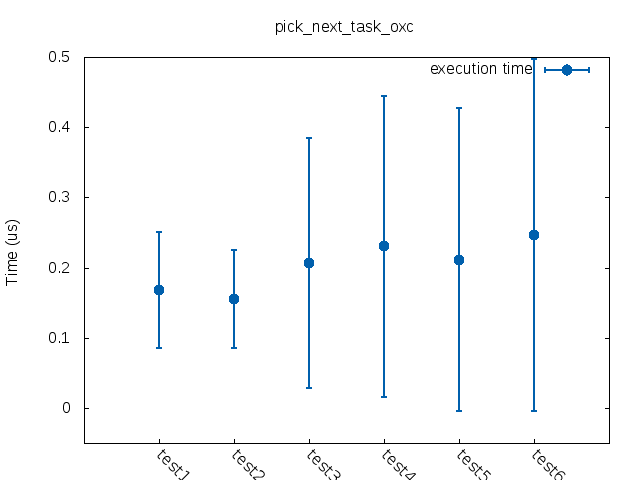
\includegraphics[width=\textwidth, totalheight=0.4\textheight]{images/pick_next_task_oxc}
        \caption{Measured execution time for \texttt{pick\_next\_task\_oxc}}
        \label{fig:pick_next}
\end{figure}
\begin{figure}[H]%htbp]
        \centering
        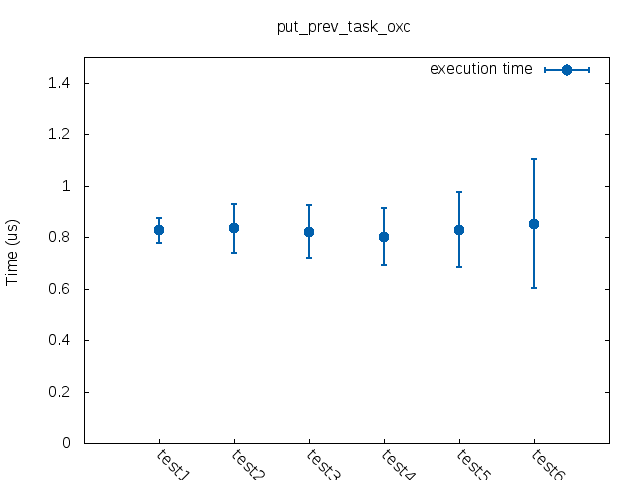
\includegraphics[width=\textwidth, totalheight=0.4\textheight]{images/put_prev_task_oxc}
        \caption{Measured execution time for \texttt{put\_prev\_task\_oxc}}
        \label{fig:put_prev}
\end{figure}
\begin{figure}[H]%htbp]
        \centering
        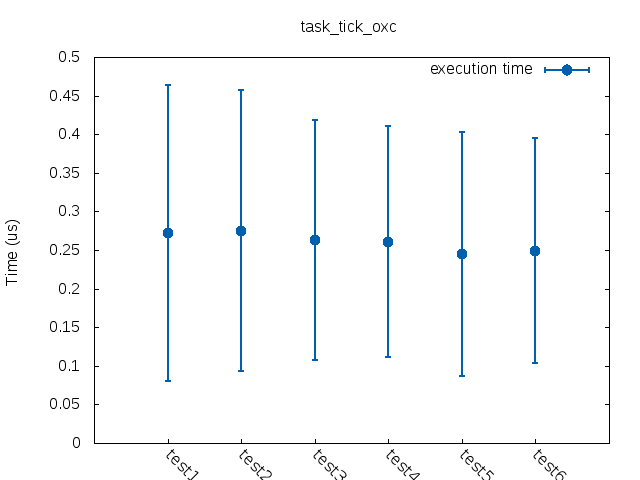
\includegraphics[width=\textwidth, totalheight=0.4\textheight]{images/task_tick_oxc}
        \caption{Measured execution time for \texttt{task\_tick\_oxc}}
        \label{fig:task_tick}
\end{figure}

Figure~\ref{fig:pick_next} shows the statistical result of 
\texttt{pick\_next\_task\_oxc} in each test. One observation from the figure
is that with more ox containers joining the system, the time spent on executing
the function codes fluctuates more. This trend also reflects in the
results for \texttt{put\_prev\_task\_oxc}, as in figure \ref{fig:put_prev}.
However, figure \ref{fig:task_tick} for \texttt{task\_tick\_oxc} does not 
show this pattern.

Now we are going to probe why the execution time of~\texttt{task\_tick\_oxc}
is more stable than the result of the other two. A look at the body of the
three functions in listing~\ref{lst:pick_next_task_oxc}, 
\ref{lst:put_prev_task_oxc} and~\ref{lst:task_tick_oxc}, we can find that 
except for the enclosed scheduling
operations, other codes in the three functions are actually the same:
to update the runqueue and the current ox container's runtime information. 
So, the different variance behaviour in measured execution time for oxc 
functions is very likely to be caused by the performance fluctuation of 
sheduling operations when they happen inside the oxc container. 

The three encapsulated scheduling operations \texttt{pick\_next\_task\_rt}, 
\\\texttt{put\_prev\_task\_rt} and \texttt{task\_tick\_rt} are defined in
RT scheduling class. Specifically, the codes of \texttt{task\_tick\_rt},
which is called inside oxc function \texttt{task\_tick\_oxc}, is listed 
below. This is a very simple function. If people read the other two
scheduling operations' codes in \emph{linux/sched/rt.c}, this function is 
still less complex in dealing with runqueues and tasks. When scheduling 
operations are called inside an ox container, there will be extra cost 
because the raw implementation details, and such an influence may 
be smaller when the scheduling operation itself is simple. This explains 
why the result in~\ref{fig:task_tick} is stable in both mean value and 
standard variance.

\begin{lstlisting}[language=C,
			caption={The simple body of \texttt{task\_tick\_rt}},
			label={lst:task_tick_rt}]
static void 
task_tick_rt(struct rq *rq, struct task_struct *p, int queued)
{
        update_curr_rt(rq);

        watchdog(rq, p);

        /*
         * RR tasks need a special form of timeslice management.
         * FIFO tasks have no timeslices.
         */
        if (p->policy != SCHED_RR)
                return;
        /*
         * The left part has no effects in our tests.
         */
        ...

}
\end{lstlisting}

\section{Experiment B}

\subsection{Experiment design}

The aim of this experiment is to estimate the overall overhead in oxc 
framework through comparison with non real-time CPU bandwidth control 
mechanisms that are already in Linux kernel. During tests the synthetic 
load is generated using the tbench benchmark tool. The CPU bandwidth 
allocated to tbench connections are allocated by oxc control, RT 
throttling and CFS bandwidth control individually. The tbench throughput 
results of oxc framework are then compared with RT throttling and CFS 
bandwidth control. By such comparisons, the overhead introduced by oxc 
control is then evaluated in a relative way.

Two tbench connections will be set up in the system.
Each connection will be dedicated to one CPU.
Without constraints, they will consume all CPU time.
In the experiment, the CPU bandwidth allocated to tbench traffic is restricted.
The per CPU bandwidth parameter used in tests includes
$0.05s/1s$, $0.1s/1s$, $0.2s/1s$, $0.4s/1s$, $0.6s/1s$ and 
$0.8s/1s$. 
Note that these are the per CPU bandwidth that is planned to assign to 
tbench tasks. Each CPU bandwidth control mechnism will restrict the 
tbench execution not exceed the configured value. And the throughput 
results will be inversly proportional to the overhead in each bandwidth 
control mechanism.

When RT throttling is tested, tbench clients and servers will be 
scheduled as RT tasks with policy \texttt{SCHED\_RR}. 
%Otherwise the client and server in the same connection cannot run at all. 
Correspondingly, to 
compare with RT throttling, tbench threads inside the ox container will 
be set as RT tasks with \texttt{SCHED\_RR} policy too. 
When comparing the oxc control with CFS bandwidth control, the tbench
threads inside ox containers will run as normal tasks. 

\subsection{Experiment results}

The thrughput results are shown in table~\ref{tab:expB1} and~\ref{tab:expB2}.

\begin{table}[H]%thbp]
	\centering
	\begin{tabular}{|l||c|c|}\hline
		 per CPU bandwidth & RT throttling & oxc control + RT scheduling\\\hline
			0.05s/1s &	21.9335	&	18.5313	\\\hline 
			0.1s/1s &	43.5794 &	36.89324 \\\hline
			0.2s/1s &	92.7356 &	73.5099	\\\hline
			0.4s/1s &	172.582 &	147.806 \\\hline
			0.6s/1s &	233	&	225.72	\\\hline
			0.8s/1s &	319.297 &	297.0607	\\\hline
	\end{tabular}
	\caption{Throughputs, in Mbps/sec, under RT throttling and oxc control}
	\label{tab:expB1}
\end{table}
\begin{table}[H]%thbp]
	\centering
	\begin{tabular}{|l||c|c|}\hline
		 per CPU bandwidth & CFS bandwidth control & oxc control + CFS scheduling  \\\hline
		 0.05s/1s	& 24.8825	& 19.2151 \\\hline
		 0.1s/1s	& 52.2106	& 39.4268 \\\hline
		 0.2s/1s	& 106.226	& 77.4225 \\\hline
		 0.4s/1s	& 215.071	& 151.465 \\\hline
		 0.6s/1s	& 323.628	& 234.369 \\\hline
		 0.8s/1s	& 433.025	& 305.1 \\\hline
	\end{tabular}
	\caption{Throughputs, in Mbps/sec, under CFS bandwidth and oxc control}
	\label{tab:expB2}
\end{table}

After a glance on the two tables, it's apparent to note that the 
throughput results under CFS bandwidth control outperform the other two. 
There are two reasons for this. Firstly, the overhead brought by CFS 
bandwidth control is indeed lower than the other two mechnanisms.
Secondly, both oxc tasks and RT tasks are more greedy than CFS tasks when 
they occupy a CPU. For oxc tasks, both RT and normal tasks are lower
priority tasks. Between RT tasks and CFS tasks, the latter one is the 
lower priority task. The oxc task or RT task will not give up a CPU to 
a lower priority task until the CPU reservation is totally consumed. So 
lower priority tasks in the system are stressed more under oxc control 
or RT throttling, especially when high reservation parameters are configured. 
However, in CFS scheduling, normal tasks, with or without CPU reservation, 
can share the CPU evenly.

\begin{figure}[htbp]
        \centering
        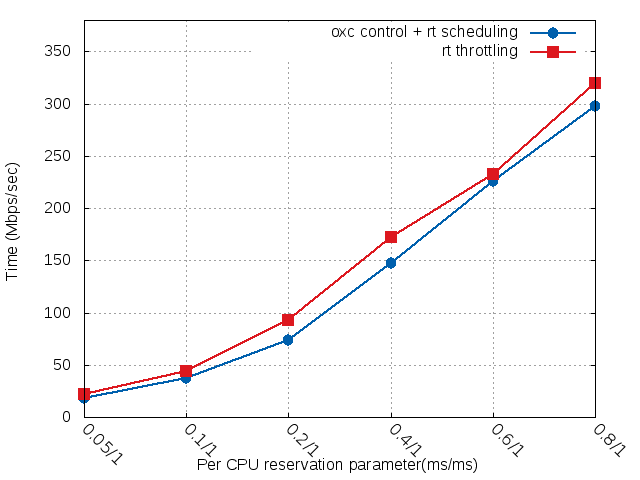
\includegraphics[width=\textwidth,totalheight=0.4\textheight]{images/expB1}
        \caption{\emph{oxc control} vs. \emph{RT throttling}}
        \label{fig:expB1}
\end{figure}

Having solved the above question, let's first study the peformance of tbench 
tasks in oxc framework when they are scheduled with \texttt{SCHED\_RR} 
policy. The comparison between oxc control and RT throttling in 
table~\ref{tab:expB1} is visualized in figure~\ref{fig:expB1}.
At first, the throughput result under RT throttling is higher and 
growing faster than the result in oxc control. However, as more CPU 
bandwdiths are reserved to tbench tasks, the throughtput results of the 
two are converging. In fact, the throughtput growing trend in oxc 
control are consistentr; yet in RT throttling, it's not like that.
When a relatively small fraction of CPU is assigned through RT throttling
and oxc control, RT throttling shows a better performance. However, with
increasing the reserved CPU bandwdith, the stress of RT throttling on
the whole system is rising too, which slows growth of the throughput. 
Under oxc control, the throughput result is almost linear with the 
given reserved bandwidth. The overhead in oxc control behaves as 
a constant factor.
This comparison gives us another meaningful implication. 
When oxc control is used, allocations of bandwidth in the system should be
cautioned so as to achieve an optimal system performance. 

The comparison between oxc control and CFS bandwidth control is shown 
in figure~\ref{fig:expB2}. As we just analyzed, CFS bandwidth control has
much better throughput results. One observation is that although with
less rasing speed, the throughput increasing trend in oxc control has the
similar shape as in CFS bandwidth control. 

\begin{figure}[htbp]
        \centering
        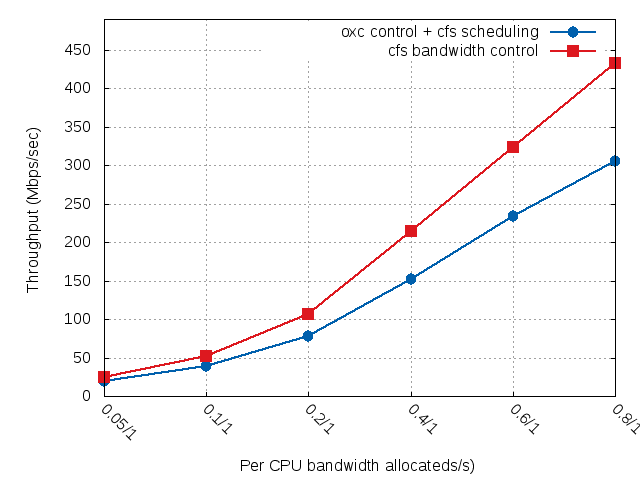
\includegraphics[width=\textwidth, totalheight=0.4\textheight]{images/expB2}
        \caption{\emph{oxc control} vs. \emph{CFS bandwidth control}}
        \label{fig:expB2}
\end{figure}
\begin{figure}[htbp]
        \centering
        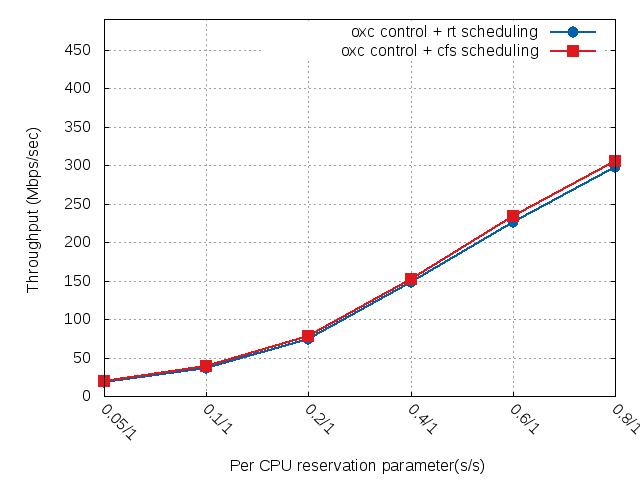
\includegraphics[width=\textwidth, totalheight=0.4\textheight]{images/expB3}
        \caption{\emph{oxc control + RT throttling} vs. \emph{oxc control + CFS scheduling}}
        \label{fig:expB3}
\end{figure}

At last, figure~\ref{fig:expB3} mixes the statistics in table~\ref{tab:expB1}
and~\ref{tab:expB2} and draws the throughput results under oxc control with
RT throttling and CFS scheduling in the same graph.
The results are quite close, and the difference can be regarded as
the scheduling cost between RT and CFS scheduling in an ox container.
Still, CFS scheduling shows better results than RT scheduling even under 
oxc framework. 
Assume, in the future, our oxc framework is fully developed and the 
degradation of modular schedulers is negligible or deterministic. 
And in such ideal conditions we get the result shown in 
figure~\ref{fig:expB3}. Such a result may demonstrate that CFS 
scheduling introduces less overhead in the system than RT scheduler. 
This is indeed one possible application of oxc framework. In some 
cases, when comparing two schedulers, we can set up the environment 
inside an ox container instead of a real machine. We can even prepare 
a certain number of ox containers to simulate a lightweight networked 
testbed. 

\section{Experiment feedbacks}

The experiment does not show that the performance of oxc control is 
better than existing bandwidth control methods. This is also not the 
experiment objective ( the comparison result with RT throttling is a 
small surprise). The experiment outcome has an unstated meaning for 
future development of oxc framework. Experiment A gives precise 
measurement of oxc function execution time and confirms the necessity 
to improve implementation quality of the oxc framework.
In experiment B, the overall performance of oxc framework is compared 
with RT throttling and CFS bandwidth control. Its experiment analysis 
shows us that how to distribute CPU bandwidth will affect both the work 
inside an ox container and the whole system behaviour; it also raises 
one possibility for oxc framework's future use. These feedbacks would 
be considered in the evolvement of the oxc framework.

%%% Local Variables: 
%%% mode: latex
%%% TeX-master: "main"
%%% End: 

\chapter{Conclusions and Future Work}



%%% Local Variables: 
%%% mode: latex
%%% TeX-master: "main"
%%% End: 


\bibliographystyle{ieeetr}%{plain}
\bibliography{biblio}

\end{document}

%%% Local Variables: 
%%% mode: latex
%%% TeX-master: t
%%% End: 
